%\documentclass{beamer}
\usetheme{MinimalGreen/beamerthemeMinimalGreen}
\usepackage{hyperref}
\usepackage[utf8]{inputenc} % this is needed for german umlauts
\usepackage[english]{babel} % this is needed for german umlauts
\usepackage[T1]{fontenc}    % this is needed for correct output 
                            % of umlauts in pdf
\usepackage{graphicx}
\usepackage{braket}
\usepackage{listings}

% "mbeq": must be equal
\newcommand{\mbeq}{\overset{!}{=}}

\begin{document}

\title{Spin Networks for Perfect State Transfer}
\author{dln-dev}
\date{5. April 2016}

\frame{\titlepage}

\section{Introduction}
\subsection{Motivation}
\begin{frame}{Hardware}
	\begin{columns}[T]
		\begin{column}{0.33\textwidth}
			\centering
   			Processors
   			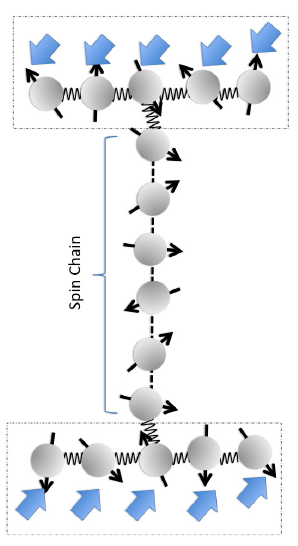
\includegraphics[width=\textwidth]{Images/processor}
		\end{column}
		\uncover<2->{\begin{column}{0.33\textwidth}
			\centering
    		Computers
    		\includegraphics[trim=0 0 0 -40mm, width=\textwidth]{Images/computer}
		\end{column}}
     	\uncover<3->{\begin{column}{0.33\textwidth}
     		\centering
     		Computing
     		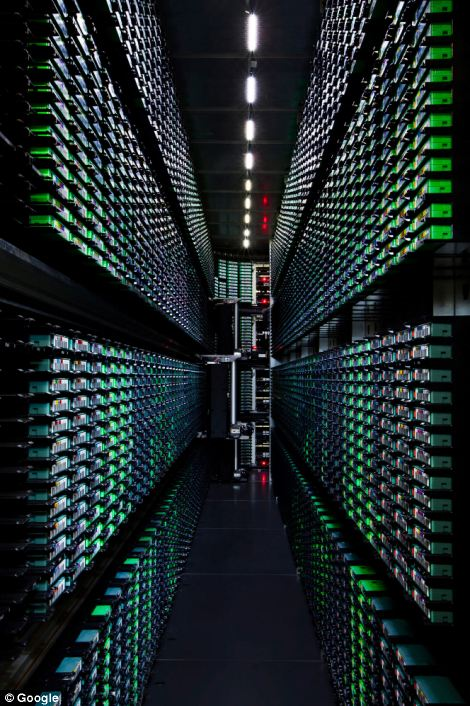
\includegraphics[trim=0 0 0 -20mm, width=\textwidth]{Images/computing}
		\end{column}}
	\end{columns}
\end{frame}

Quantum processors work on quantum registers. These are highly controlled regions with an intricate machinery of manipulators controlling the state of the qubit itself (preparation/initialization) as well as the qubit couplings. These controls will introduce quite some noise into the system which makes it necessary to separate controlled parts of the system by less controlled, mostly passive parts. In these parts, state transfer has to happen with acceptable fidelity.\\
Quantum computers themselves might consist of several quantum processors working in parallel, similar to present aproaches to computing using massive parallelization for increased computation power.\\
The first feasible real world implementation of a public-access quantum computer would probably follow a cloud-like model, where a huge computing facility would provide access to several available quantum computers via a web interface. The received states would need a means of transportation to available sites realizing some form of load balancing.\\
One might question, though, in how far these approaches are different at all. Many proposals for realizable quantum computers suggest distributed registers, sometimes containing only as few as two controllable qubits separated by some form of state transfer capable spacers. In a setting like this, splitting and distributing a computation to certain registers solves all the above mentioned problems at once. Different register regions are chosen for different processes, regardless of spacial distance. Yet, these registers would need connectivity in the form of state transfer capable network. 

\subsection{Requirements}
\begin{frame}{Requirements}
	\begin{itemize}
		\item Separation of highly controlled regions
		\item Spacers
		\begin{itemize}
			\item (Perfect) state transfer
			\item Fixed interactions
			\item Natural dynamics
			\item Control single qubit at each end only (for now)
		\end{itemize}
	\end{itemize}
	
	$\rightarrow$ Spin networks!
%Registers are highly controlled regions (gates, ...), probably need separation, spacers need to be capable of state transfer -> spins, control free region: permanent, fixed interactions between spins, natural dynamics (initialize, wait, read); For now: only single qubits control at each site, homogenous constant couplings, PST (Explain!), spin networks instead so no transformation is needed.
\end{frame}

The aforementioned requirements suggest a medium similar to what the quantum registers are made of, so that no conversion, e.g. from solid state registers to photons is necessary. We will restrict ourselves here to perfect state transfer, fixed interactions and natural dynamics. Control over these spacers is then reduced to initialization, initial state transfer (perhaps in the form of a SWAP gate operation) and procession of the received qubit. At each site, only a single qubit shall be controlled. Other options will be explored at a later time. \\
A natural suggestion for a realization would be networks of two-level systems comprising qubits themselves. Therefore, we will investigate the feasability of spin networks as quantum state transfer enablers. This is called spin chain engineering.

\subsection{Model}
\begin{frame}[t]{Model}	
	\begin{exampleblock}{}
	\setlength\abovedisplayskip{-8pt}
	\begin{center}
		\[H_{XX}=\frac{1}{2}J\sum_{i=1}^{N}{\left[\sigma_i^x\sigma_{i+1}^x + \sigma_i^y\sigma_{i+1}^y\right]}\]
	\end{center}
	\end{exampleblock}
	\begin{itemize}
		\item $J\equiv const.$
		\item No z coupling
		\item $\left[H_{XX},\sigma^z_\text{tot}\right] = 0$
		\item Eigenstates: $\ket{\tilde{k}} = \sqrt{\frac{2}{N+1}}\sum_{s=1}^N\sin\left(\frac{\pi ks}{N+1}\right)\ket{s}$
		\item Eigenvalues: $ E_k = 2\cos\left(\frac{\pi k}{N+1}\right)$
	\end{itemize}
%    Show complete Heisenberg model (no local potentials), explain terms, why no z coupling etc., commutes with total z spin, then XY model, what do states look like?
\end{frame}

The model we are using is a reduced version of the Heisenberg model. We assume x- and y-component spin interaction only and omit z-interaction completely for computability reasons. z-interactions do not pose problems in principal right now, since we will look at single spin excitations only for now. Further, we will assume homogeneous (same coupling between every qubit) and isotropic couplings (same coupling for x- and y-component respectively). This is called the XX-model. Other configurations are no principal hindrance, but these rather loose assumptions make an introduction to this topic much easier.\\
The total z-spin operator commutes with the hamiltonian. Therefore, a common set of eigenvectors exists. The hamiltonian consequently can be decomposed into several smaller subspaces each belonging to a specific eigenvalue of the total z-spin operator. The dynamics of a state belonging to one such subspace will therefore stay in the specific subspace. A state belonging to the single spin subspace will evolve into a superposition of single spin states.\\
The eigenstates can be calculated by diagonalizing the hamiltonian or analyzing states on a ferromagnetic chain. Low energetic excited spin waves are superpositions of all single spin up states (assuming periodic boundary conditions at the moment). Sharply localized single spin states can be constructed as superpositions of these spin wave states. These are sometimes called twisted-w states in quantum information science. The term seems to stem from Fourier analysis of radio signals.

\subsection{Math setup}
\begin{frame}{Math setup}
	\begin{description}
	\item [Ground state of ferromagnetic spin-$\frac{1}{2}$ chain:] \[ \ket{\uparrow}_1 \otimes \ket{\uparrow}_2 \otimes \dots \otimes \ket{\uparrow}_N = \ket{\uparrow_1\uparrow_2\dots\uparrow_N} := \ket{0} \]
	\item [Excitation operator $\sigma^- = \frac{1}{2}\left(\sigma^x - \text{i}\sigma^y\right)$:] \[ \text{1}_1 \otimes \text{1}_2 \otimes \dots \otimes \text{1}_{s-1} \otimes \sigma^- \otimes \text{1}_{s+1} \otimes \dots \otimes \text{1}_N := \sigma^-_s \]
	\item [Single spin excitation:] \[ \sigma^-_s\ket{0} := \ket{s} \]
	\item [Single spin superposition:] Prepare spin at $s$ as $\alpha\ket{\uparrow}_s + \beta\ket{\downarrow}_s \rightarrow$ \[ \ket{\Psi} := \alpha\ket{0} + \beta\ket{s} \]
	\end{description}
%    Explain numbers as kets, superpositions, graphs, later binary scheme for graphs, adjacency matrices and correspondence to hamiltonian, fidelity.
\end{frame}

In short, states as well as operators are contructed by the tensor product, in the latter case involving many unity matrices of dimension 2. There is a direct correspondence of the order of operations and the numbering of spins in the considered system.

\begin{frame}{Perfect state transfer}
%	In general, target state will evolve into a mixed state:\\
	\[ \ket{\Psi_{in}} = \cos{\left(\frac{\Theta}{2}\right)} \ket{0} + e^{\text{i}\Phi}\sin{\left(\frac{\Theta}{2}\right)}\ket{s} \]
	\[ \ket{\Psi_{out}} = \frac{1}{\sqrt{P(t)}}\left( \cos{\left(\frac{\Theta}{2}\right)} \ket{0} + e^{\text{i}\Phi}\sin{\left(\frac{\Theta}{2}\right)}f^N_{r,s}(t)\ket{r} \right) \]
	\[ \rho_{out} = P(t)\ket{\Psi_{out}}\bra{\Psi_{out}} + \left( 1-P(t) \right)\ket{\uparrow}\bra{\uparrow} \]
%	and
%	\[ P(t) = \cos^2{\left(\frac{\Theta}{2}\right)} + \sin^2{\left(\frac{\Theta}{2}\right)}\lvert f^N_{r,s}(t)\rvert^2 \]
	Transition amplitude: $f^N_{r,s}(t) = \bra{r}e^{\text{i}H t}\ket{s}$\\
	\begin{exampleblock}{Fidelity:}
	\setlength\abovedisplayskip{-8pt}
	\begin{center}
		\[ \mathfrak{F}(t) = \frac{1}{4\pi}\int \!\bra{\Psi_{in}}\rho_{out}\ket{\Psi_{in}} \, \mathrm{d}\Omega = \frac{\lvert f^N_{r,s}\rvert\cos{\lambda}}{3} + \frac{\lvert f^N_{r,s}\rvert^2}{6} + \frac{1}{2}\]
% in order to give qualitative statements it suffices to know f^N_r,s
	\end{center}
	\end{exampleblock}
\end{frame}

In general, the target qubit will evolve into a mixed state. The expression for the state description is easily calculated by applying the time development operator, expressed as its eigenvector-eigenvalue decomposition, to the pure state. Since there is no development of the ground state involved (this is the only state in the ground state subspace), there is only a term influencing the excited part of the state. This term in general will have an absolute less than one. The state therefore will in general not directly lie on the Bloch sphere, but inside it as a mixed state.\\
The notion of fidelity comes from the density matrix associated with the target system averaged over all pure input states. It turns out, however, that for the fidelity of state transfer to equal unity, it is enough to ensure the absolute of the transition amplitude to be unity. The overall phase in form of the cosine can be neutralized by an overall magnetic field. We will restrict ourselves here to ensuring the unit absolute of the transition amplitude.\\
There are other forms of quantisizing the quality of state transfer such as concurrence or von-Neumann entropy. The fidelity as defined here is the most widely adopted.

\begin{frame}[t]{Graphs}
	\begin{exampleblock}{}
	\setlength\abovedisplayskip{-8pt}
	\begin{center}
		$G = (V,E)$
	\end{center}
	\end{exampleblock}
	\begin{itemize}
		\item Edges undirected $\rightarrow E \subseteq \{\{i,j\}\colon i,j \in V\}$
		\item Single edges only $\rightarrow \{i,j\}$ unique
	\end{itemize}   
%	is a subset of the set of all unordered pairs of vertices in $V$.
	Example: $V = \{1,2,3\}, E = \{\{1,2\},\{2,3\}\}$
		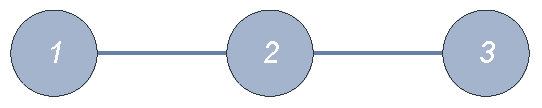
\includegraphics[trim=0 0 0 -5mm, width=\textwidth]{Images/chain3}
\end{frame}

Graphs are great tools for not only visualizing, but also analyzing spin networks in general. Vertices symbolize qubit sites, edges connect qubits between which exchange interaction occurs. As such, edges have to be undirected and unique, since exchange interaction is symmetric. It is natural therefore to define edges as unordered pairs of vertices. Note that the vertices inside edges do not necessarily have to be different. These would amount to self-interaction. Their representation in graphs would be self-loops at the respective vertices.

\begin{frame}[t]{Adjacency Matrices}
	\begin{exampleblock}{}
	\setlength\abovedisplayskip{-8pt}
	\begin{center}
		$a_{ij} = \left\{
	\begin{array}{ll}
		1  & \{i,j\} \in E \\
		0  & \text{otherwise}
	\end{array}
\right.$	
	\end{center}
	\end{exampleblock}
	\begin{itemize}
		\item No multi-edges $\rightarrow$ all elements either $0$ or $1$
		\item Unordered Pairs $\rightarrow$ symmetric
		\item Orthogonal basis exists, eigenvalues are roots of $det(A-\lambda \text{1}) = 0$
	\end{itemize}
	\begin{columns}[T]
		\begin{column}{0.5\textwidth}
			\centering
   			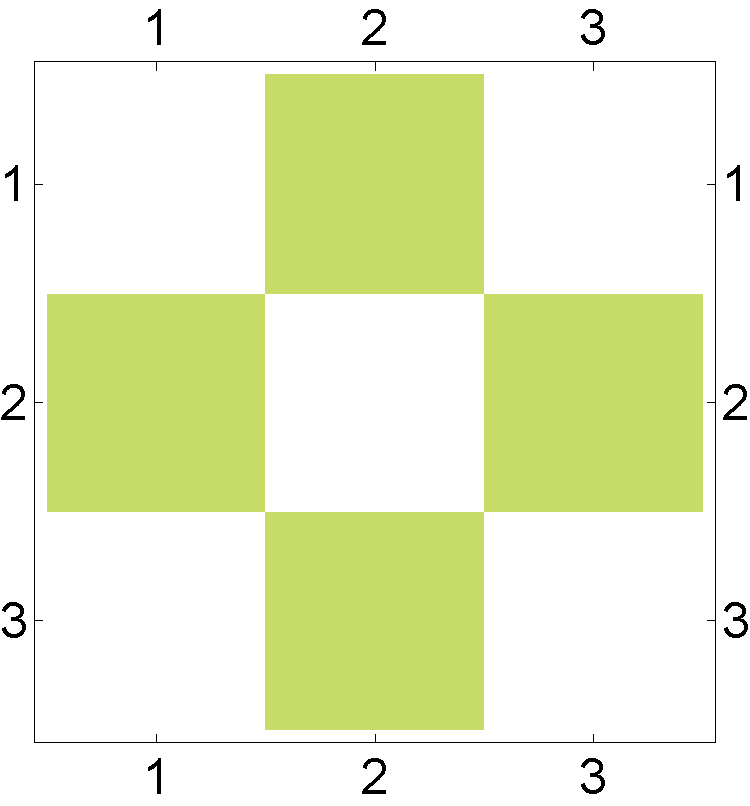
\includegraphics[trim=0 0 0 5mm, width=0.5\textwidth]{Images/adj_chain3}
		\end{column}
		\begin{column}{0.5\textwidth}
			\centering
    		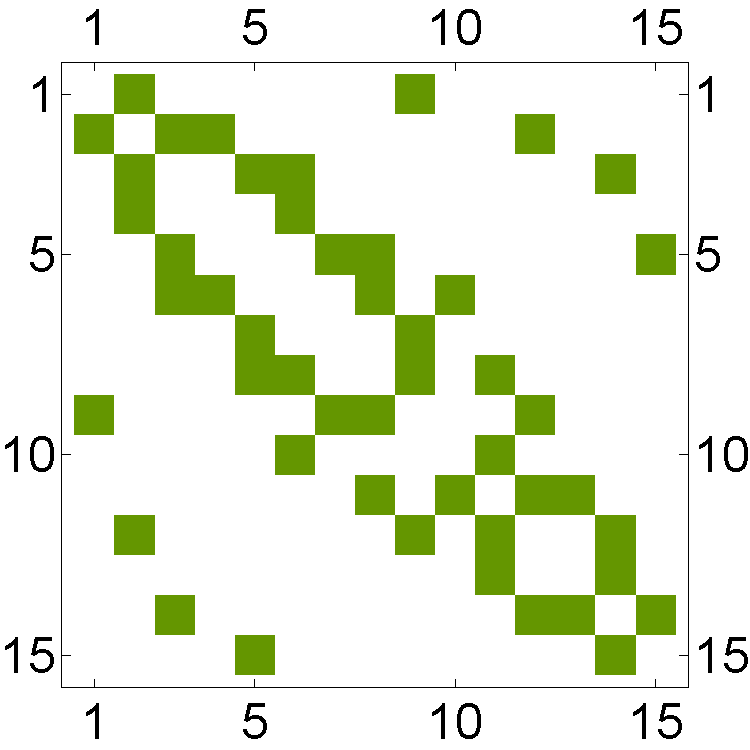
\includegraphics[trim=0 0 0 18mm, width=0.6\textwidth]{Images/adj_ring6_2}
		\end{column}
	\end{columns}
\end{frame}

An algebraic treatment of graphs is made possible by adjacency matrices. These encode the edges of a graph by interpreting rows and columns as vertices. If there is a connection between qubit 1 and 2, there will be a 1 in row 1, second column or zero  otherwise. Edges are unordered sets and the adjacency matrix therefore symmetric. The consequence of this is that there exists a set of orthogonal eigenvectors which will be important in a proof later on.\\
The examples here are the adjacency matrices of a 3-qubit chain and the 2-spin subspace representation graph of a 6-qubit ring.

\begin{frame}{Correspondence to Hamiltonians}
	\begin{columns}[T]
		\begin{column}{0.33\textwidth}
			\centering
   			6-qubit ring
   			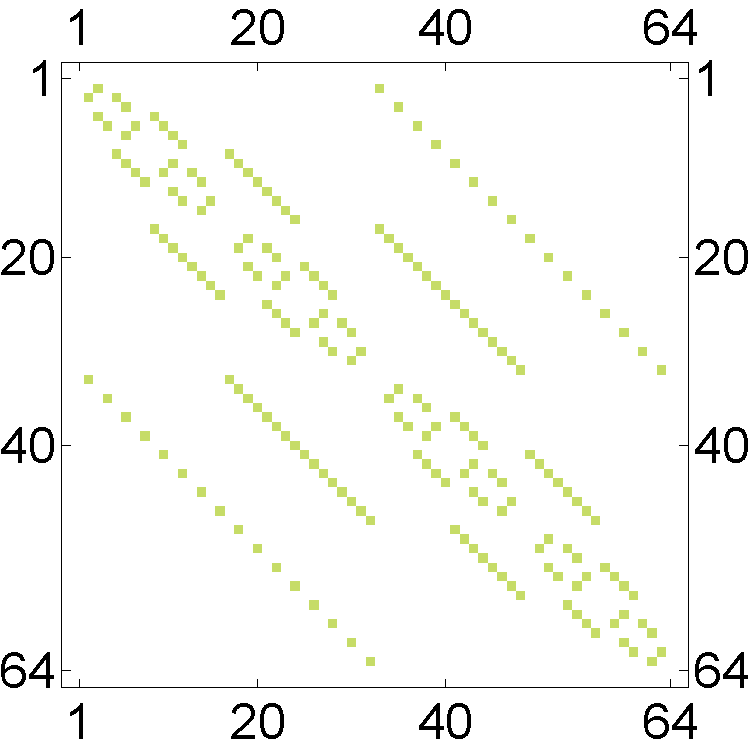
\includegraphics[width=\textwidth]{Images/ring6_hamilton}
		\end{column}
		\uncover<2->{\begin{column}{0.33\textwidth}
			\centering
    		Graph
    		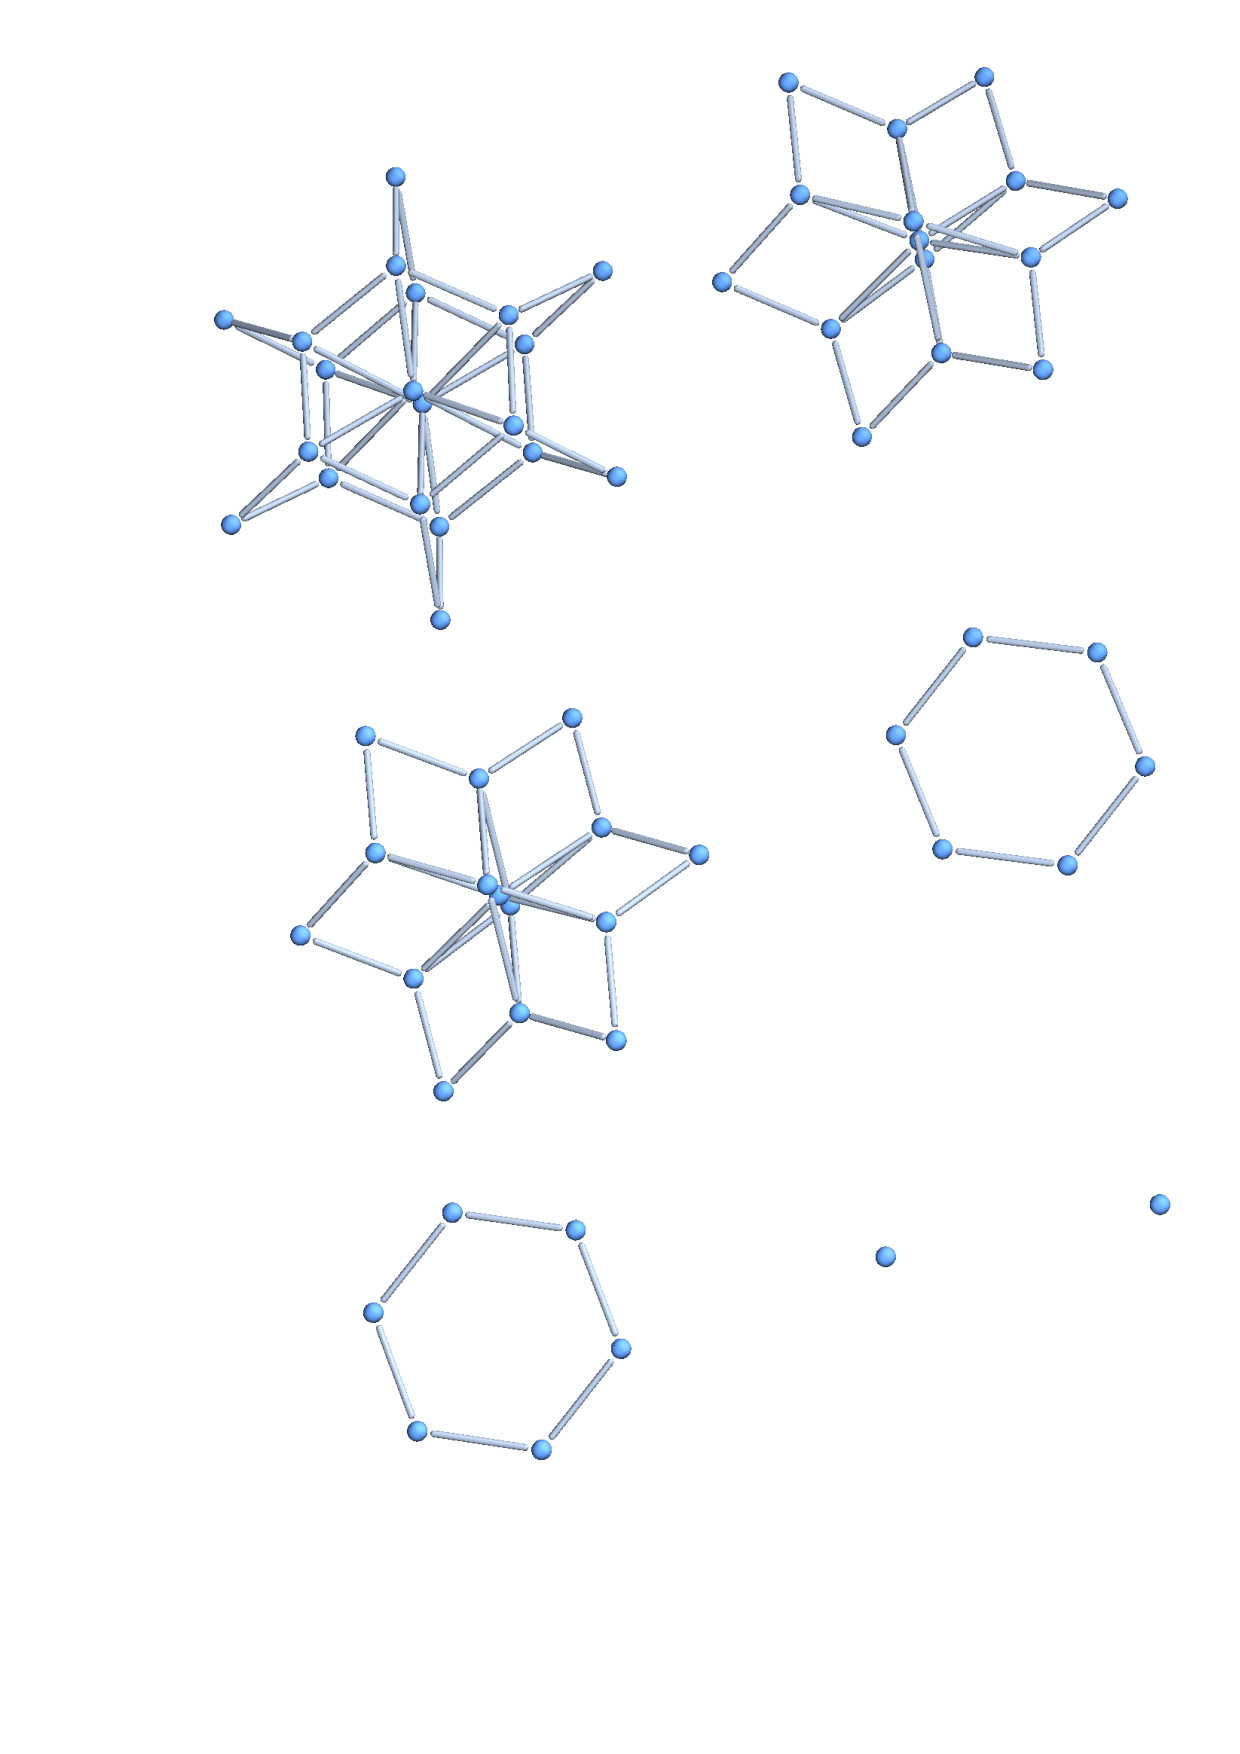
\includegraphics[trim=0 0 0 0mm, width=\textwidth]{Images/ring6_hamilton_graph3d}
		\end{column}}
     	\uncover<3->{\begin{column}{0.33\textwidth}
     		\centering
     		Single spin subspace
     		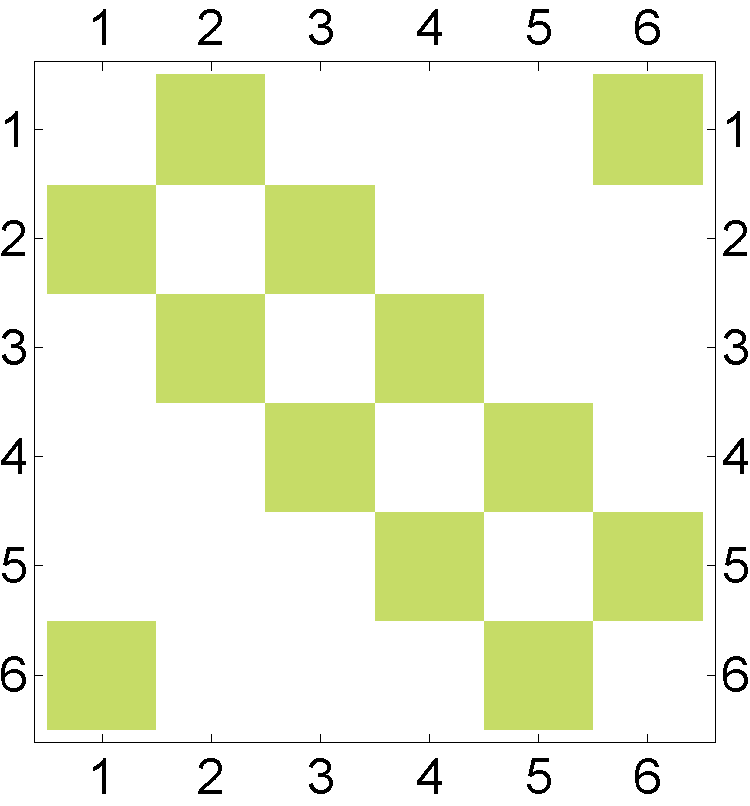
\includegraphics[trim=0 0 0 0mm, width=\textwidth]{Images/adj_ring6_1}\\
     		\uncover<4->{This is the adjacency matrix for the 6-qubit ring!}
		\end{column}}
	\end{columns}
\end{frame}

\begin{frame}{How to identify subspaces}
	\begin{columns}[T]
		\begin{column}{0.5\textwidth}
			\centering
   			Recipe:
   			\begin{itemize}
   				\item Matrix labels $-1$
   				\item Convert labels to binary
   				\item Identify rows and columns with equal number of $1$s (e.g. 1)
   				\item Strip off all other rows and columns
   				\item Compile matrix from rows and columns left
   				\item ${N \choose s}$ vertices (states) in graph
   			\end{itemize}
   		\end{column}
		\begin{column}{0.5\textwidth}
			\centering
    		Graph
    		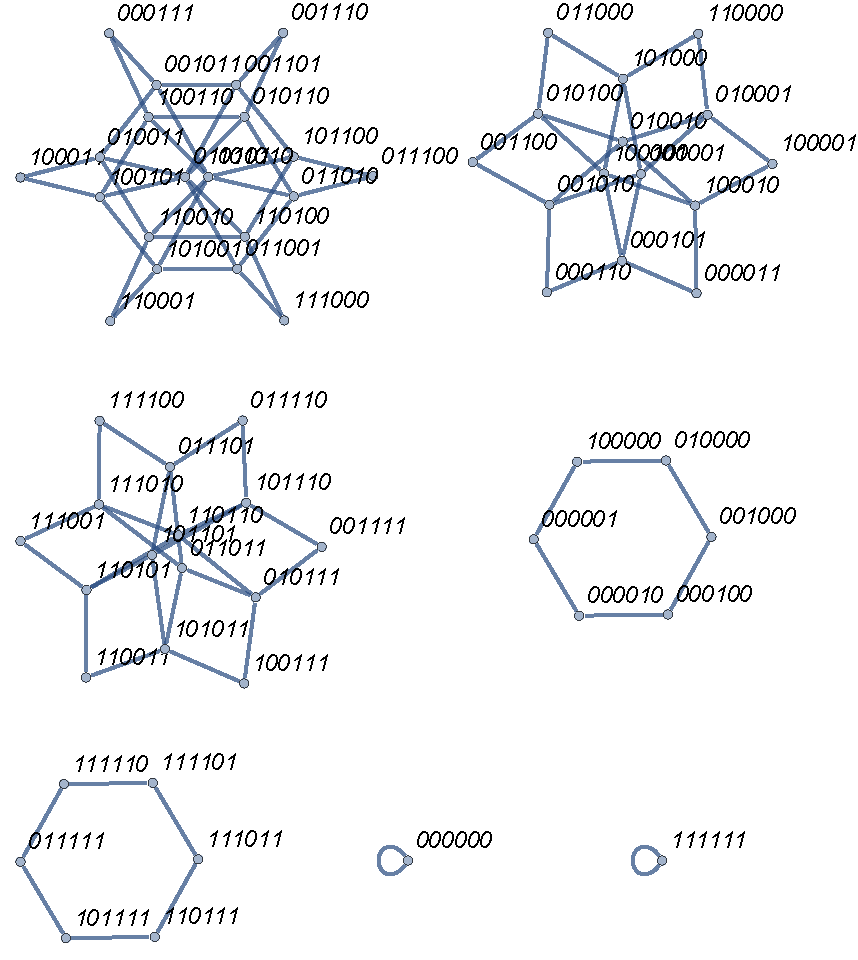
\includegraphics[trim=0 0 0 0mm, width=\textwidth]{Images/ring6_hamilton_graph3d_alt}
		\end{column}
	\end{columns}
\end{frame}

Hamiltonians are adjacency matrices. This is due to how they are built up by the Pauli matrices. Next neighbours are represented by Pauli matrices with neighbouring indices, creating an entry of 1 in case there is a connection. This also causes (in the case of chains) an ordering that enables one to easily identify rows and columns belonging to certain subspaces by using binary numbers. A 1 in this binary representation corresponds to an excited spin at the location in the chain corresponding to the location in the bitstring. All rows and columns represented as a binary number with a fixed number of 1s therefore belong to the subspace of z-spin equal to the number of 1s.

\begin{frame}[t]{Cartesian Product of Graphs}
	\begin{exampleblock}{}
	\setlength\abovedisplayskip{-8pt}
	\begin{center}
		$G \times H = (V_{G\times H},E_{G\times H})$
	\end{center}
	\end{exampleblock}
	\begin{itemize}
		\item $V_{G\times H} = V(G) \times V(H)$
		\item $\{(u,u'),(v,v')\} \in E_{G\times H}$ if 
		\begin{itemize}
			\item $u = v$ and $\{u',v'\} \in E_H$ or
			\item $u' = v'$ and $\{u,v\} \in E_G$
		\end{itemize}
	\end{itemize}
	\begin{exampleblock}{}
	\setlength\abovedisplayskip{-8pt}
	\begin{center}
		$A_{G\times H} = A_G \otimes \text{1}_{\left|V_H\right|} + \text{1}_{\left|V_G\right|} \otimes A_H$
	\end{center}
	\end{exampleblock}
\end{frame}

\begin{frame}{Examples of Product Graphs}
	\begin{columns}[T]
		\begin{column}{0.33\textwidth}
			\centering
   			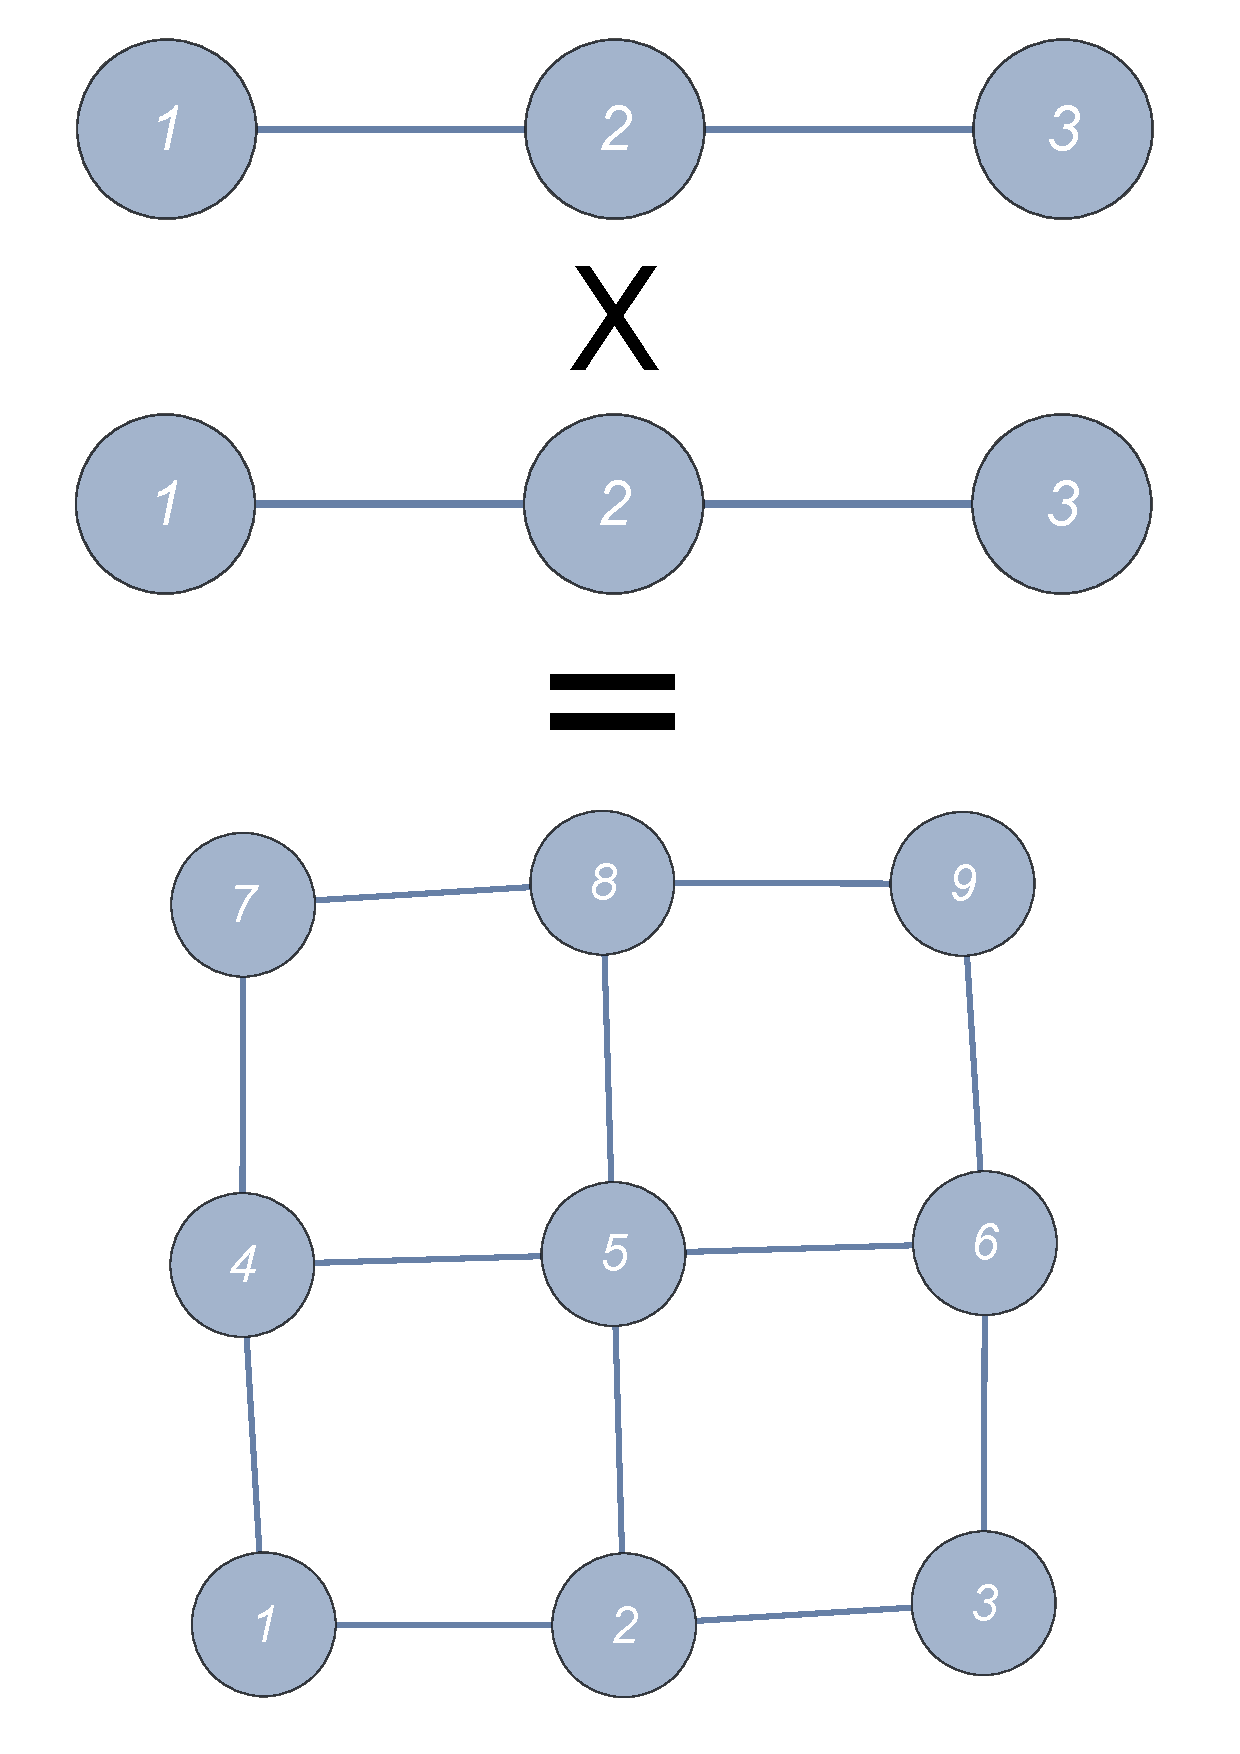
\includegraphics[width=\textwidth]{Images/graphprod_chain3_square}
		\end{column}
		\uncover<2->{\begin{column}{0.33\textwidth}
			\centering
    		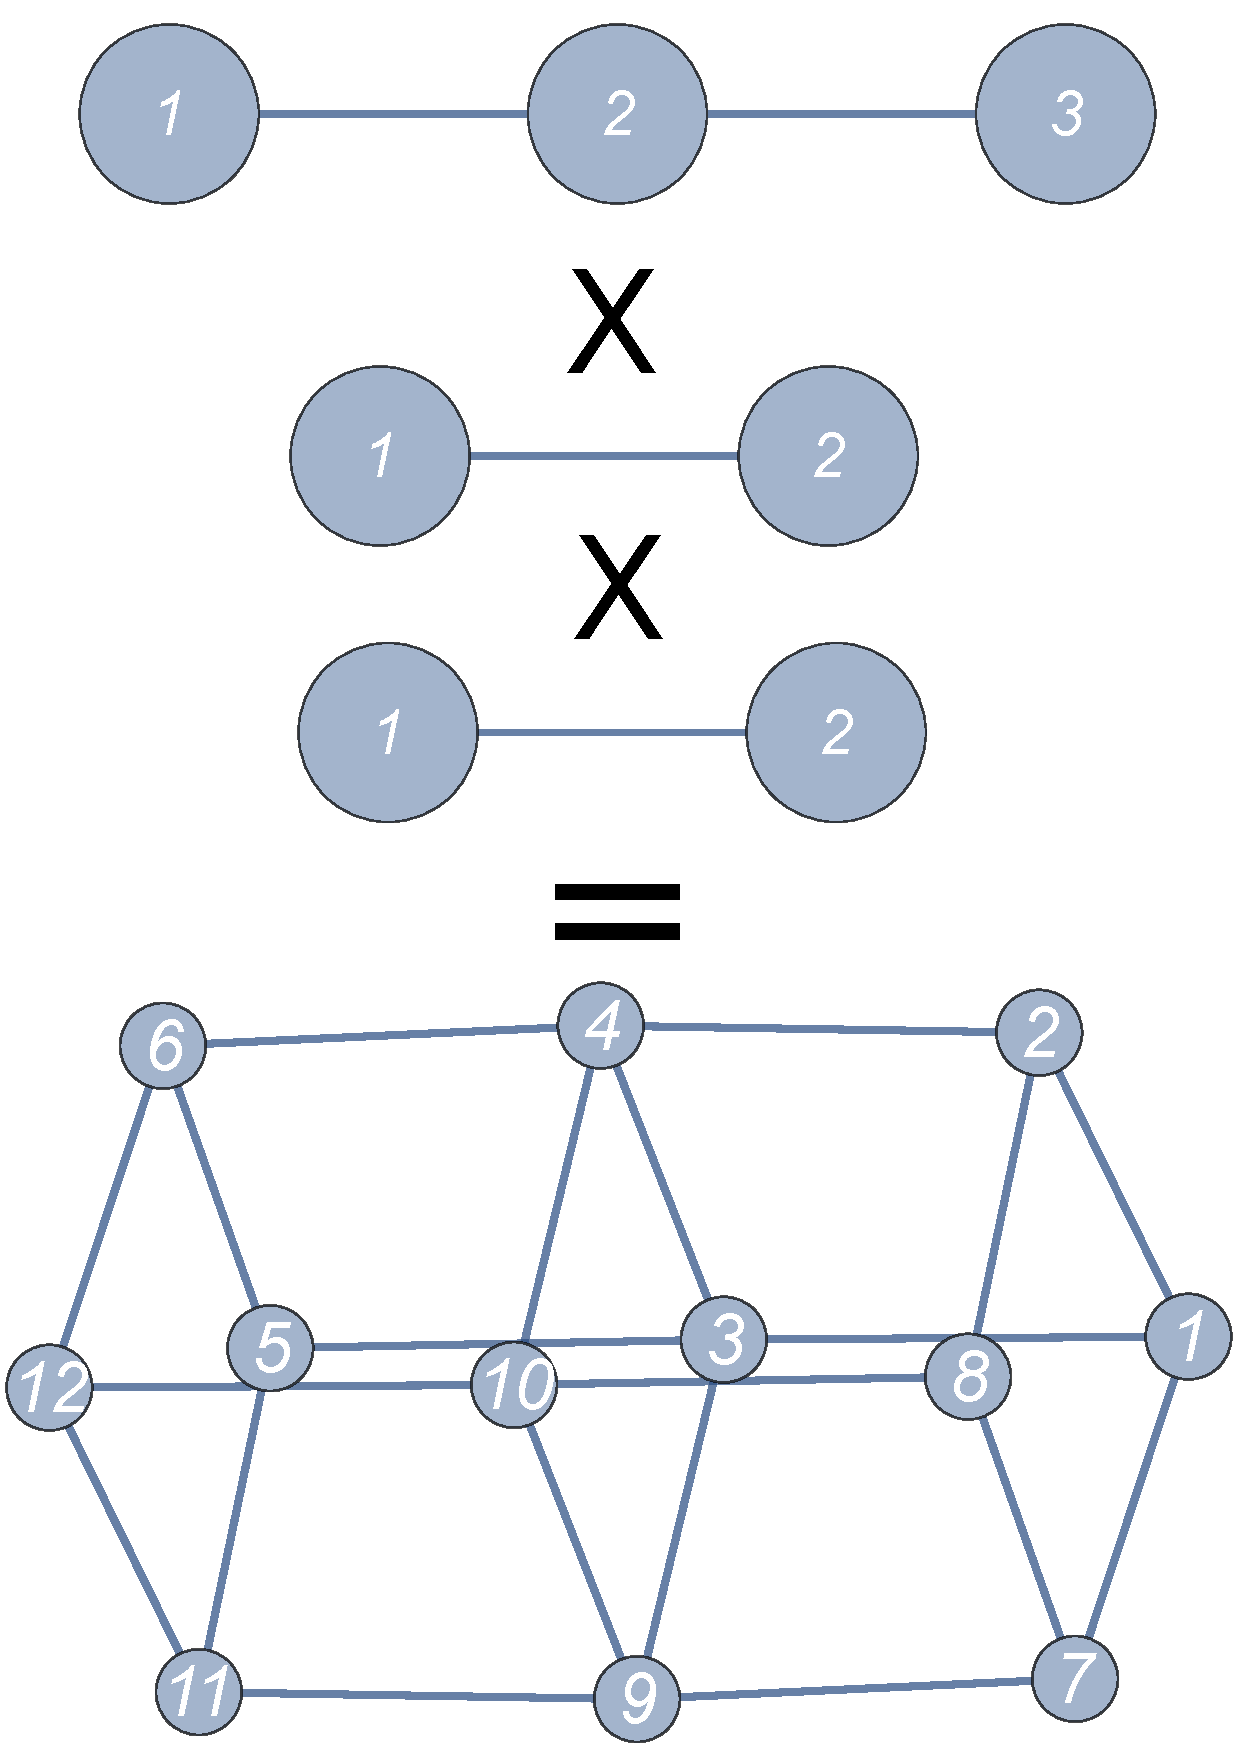
\includegraphics[trim=0 0 0 -10mm, width=\textwidth]{Images/graphprod_chain3_chain2_square}
		\end{column}}
     	\uncover<3->{\begin{column}{0.33\textwidth}
     		\centering
     		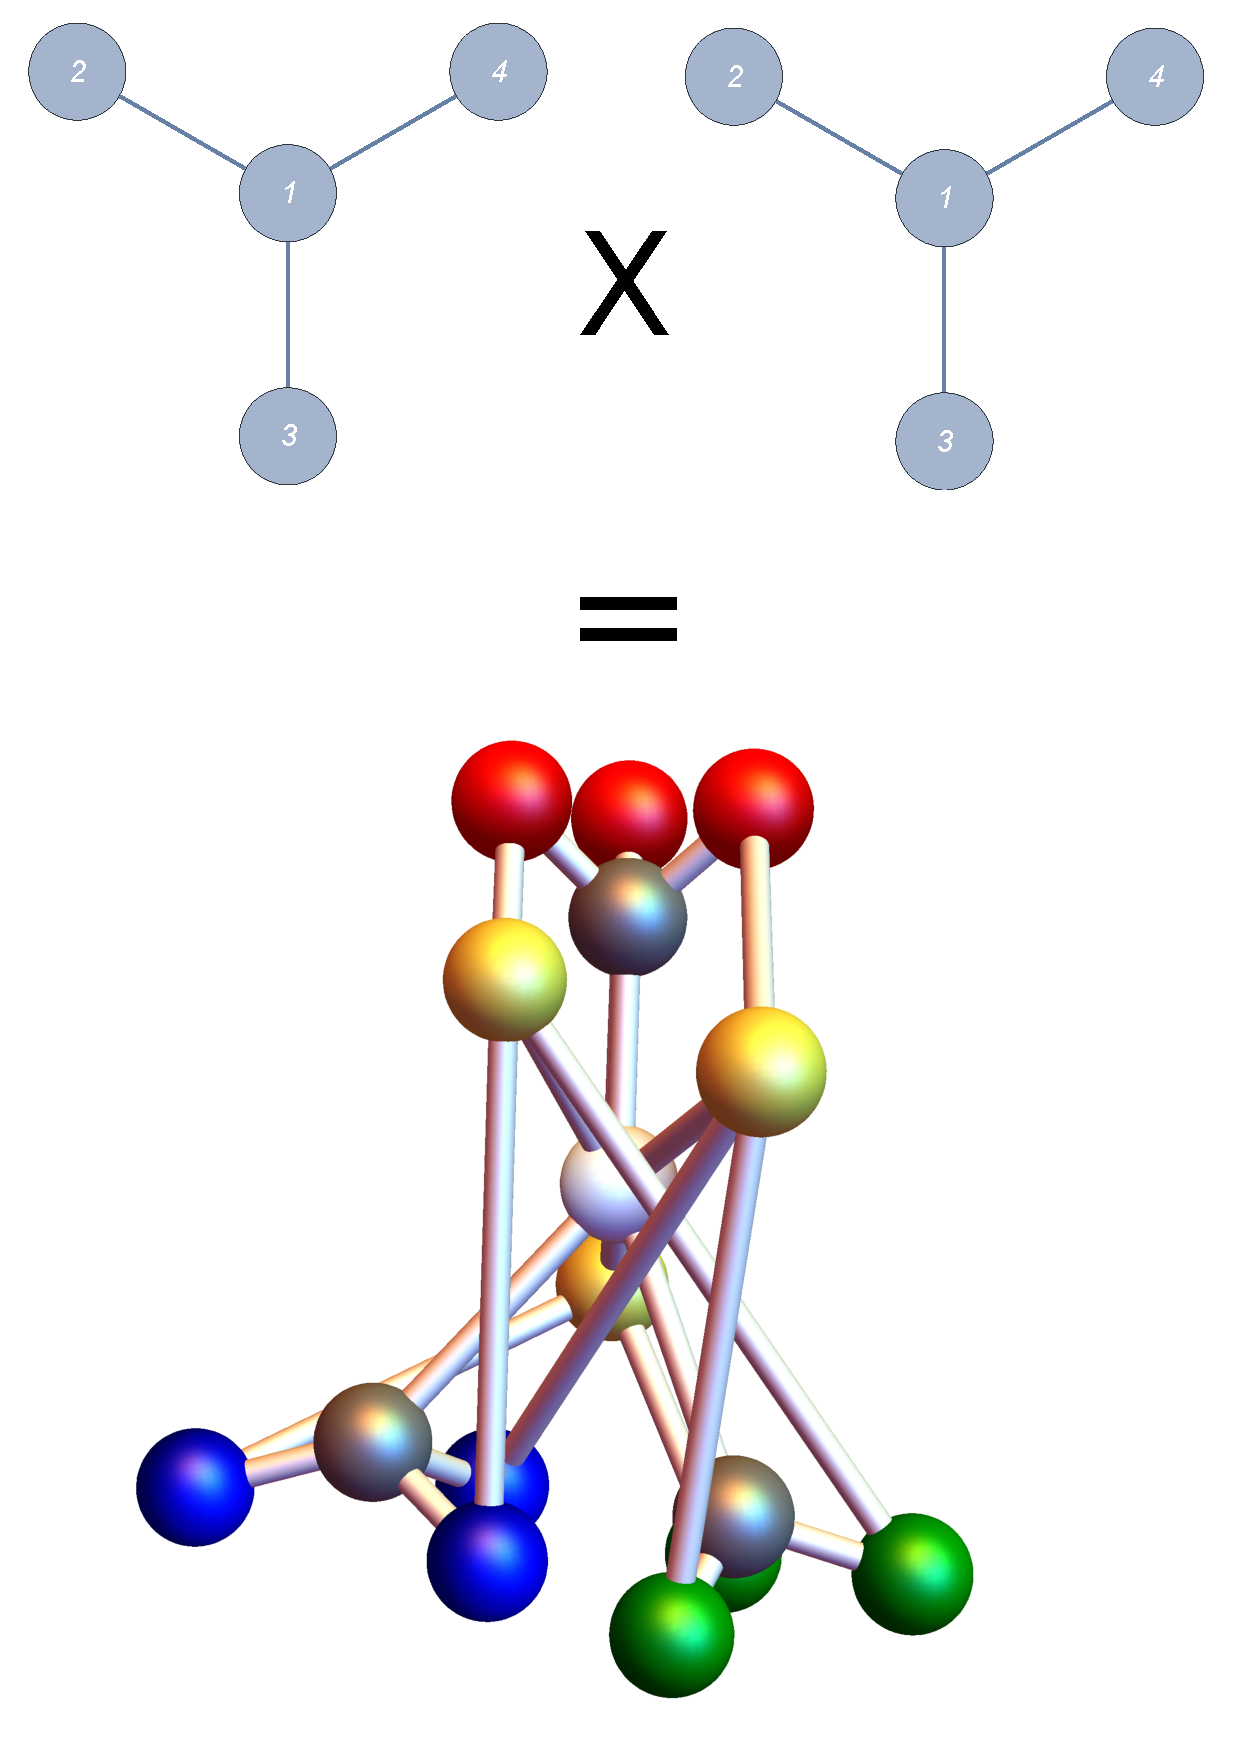
\includegraphics[trim=30mm 0 0 0, width=\textwidth]{Images/graphprod_switch_square}
		\end{column}}
	\end{columns}
\end{frame}

Higher order graphs can be built by using the cartesian product of graphs, or graph product. Note that this is not a tensor product, which can be defined for graphs as well. Vertices of the product graph are unordered pairs of underlying simple graph vertices. The graph product is therefore commutative. The edge set consists of unordered pairs of unordered vertex pairs in which either the first vertices or the second vertices are connected in one of the original graphs. In other words, if graph G has 4 vertices one would take 4 copies of graph H and connect the vertices in such a way, that these connections form G graphs. 

\begin{frame}{Fidelity on Product Graphs}
	\begin{align*}
		f^{\left|V_{G\times H}\right|}_{(r,r'),(s,s')}(t) &= \left( \bra{r} \otimes \bra{r'} \right)e^{-\text{i}A_{G\times H}t} \left( \ket{s} \otimes \ket{s'} \right) \\
		&= \left( \bra{r} \otimes \bra{r'} \right)e^{-\text{i}(A_G \otimes \text{1}_{\left|V_H\right|})t} e^{-\text{i}(\text{1}_{\left|V_G\right|} \otimes A_H)t} \left( \ket{s} \otimes \ket{s'} \right) \\
		&= \sum_{k=1}^{K}\left[ \left( \bra{r} \otimes \bra{r'} \right) \ket{g'_k}\bra{g'_k}e^{-\text{i}G_k{}'t} \ket{h_k'}\bra{h_k'}e^{-\text{i}H_k{}'t} \left( \ket{s} \otimes \ket{s'} \right) \right]
	\end{align*}
	%\begin{align*}
		%f^{G\times H}_{N\times N'}(t) &= \left( \bra{N} \otimes \bra{N'} \right)e^{-\text{i}A_{G\times H}t} \left( \ket{1} \otimes \ket{1'} \right) \\
		%&= \left( \bra{N} \otimes \bra{N'} \right)e^{-\text{i}(A_G \otimes \text{1}_{\left|V_H\right|})t} e^{-\text{i}(\text{1}_{\left|V_G\right|} \otimes A_H)t} \left( \ket{1} \otimes \ket{1'} \right) \\
		%&= \sum_{k=1}^{K}\left[ \left( \bra{N} \otimes \bra{N'} \right) \ket{g'_k}\bra{g'_k}e^{-\text{i}G_k{}'t} \ket{h_k'}\bra{h_k'}e^{-\text{i}H_k{}'t} \left( \ket{1} \otimes \ket{1'} \right) \right]
	%\end{align*}
	\begin{itemize}
		\item $K = \left|V_{G\times H}\right|$, $L = \left|V_G\right|$, $M = \left|V_H\right| \rightarrow K = L\cdot M$
		\item $\bra{g'_k} = \bra{g_l} \otimes \bra{e_m}$, $\bra{h'_k} = \bra{e_l} \otimes \bra{h_m}$ etc.
		\item $G_k{}' = G_l\cdot E_m$, $H_k{}' = E_l\cdot H_m$
		\item $(A\otimes B)(C\otimes D) = (AC)\otimes (BD)$
	\end{itemize}
	\begin{align*}
		f^{\left|V_{G\times H}\right|}_{(r,r'),(s,s')}(t) &= \sum_{l=1}^L\left[ \Braket{r|g_l}\Braket{g_l|s}e^{-\text{i}G_l t} \right] \sum_{m=1}^M\left[ \Braket{r'|h_m}\Braket{h_m|s'}e^{-\text{i}H_mt} \right] \\
		&= \Braket{r|e^{-\text{i}A_G t}|s}\Braket{r'|e^{-\text{i}A_H t}|s'}
	\end{align*}
\end{frame}

\begin{frame}[t]{Fidelity on Product Graphs}
	\begin{exampleblock}{}
	\setlength\abovedisplayskip{-8pt}
	\begin{center}
		$ f^{\left|V_{G\times H}\right|}_{(r,r'),(s,s')}(t) = f^{\left|V_G\right|}_{r,s}(t)\cdot f^{\left|V_H\right|}_{r',s'}(t) $
	\end{center}
	\end{exampleblock}
	\begin{align*}
		f^{\left|V_G\right|}_{r,s}(t) &= 1 \text{ for } t = \tau_G \\ 
		f^{\left|V_H\right|}_{r',s'}(t) &= 1 \text{ for } t = \tau_H \\ 
		f^{\left|V_{G\times H}\right|}_{(r,r'),(s,s')}(t) &= 1 \text{ for } t = \tau_{G\times H}
	\end{align*}
	\begin{exampleblock}{}
	\setlength\abovedisplayskip{-8pt}
	\begin{center}
		$ \text{iff }\frac{t_G}{t_H} \in \mathbb{Q}$ %\rightarrow t_{G\times H} = LCM(t_G,t_H) $
	\end{center}
	\end{exampleblock}
\end{frame}

The fidelity on product graphs shows a product structure. The proof exploits the additive structure of adjacency matrices of product graphs. One simply expresses the transition amplitude of the product graph in terms of the underlying graphs. The eigenvectors and eigenvalues of the original graph adjacency matrices times the identity matrix are simply the (tensor) products of each respective operators eigenvectors and eigenvalues. Applying the cartesian product reduction identity 4 times and splitting the sums reveals that the transition amplitude of state transfer on a product graph is the product of the transition amplitudes for state transfer on the underlying graphs.\\
Having a unity transition amplitude requires unit transfer times of underlying graphs to form rational numbers when divided. This is rarely the case. The obvious exclusion is the product of graphs with themselves. In this case, perfect state transfer is automatically achieved in exactly the same time. This means more distance can be covered by connecting qubits in a way so that they resemble the product graph of a simple PST graph with itself.

\section{Examples}
\subsection{Spin Chains}
\begin{frame}[t]{Spin Chains}
	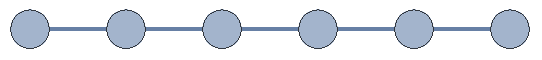
\includegraphics[trim=0 0 0 0, width=\textwidth]{Images/chain6_nolabels}\\
	\[f_{N,1}^N(t) = \frac{2}{N+1}\sum_{s}^N\sin\left(\frac{\pi s}{N+1}\right)\sin\left(\frac{\pi sN}{N+1}\right)e^{-\text{i}E_s t} \]
	\begin{itemize}
		\item $N=2$: \,\,\,\,$f_{2,1}^2(t) = -\text{i}\sin(t)$ \,\,\,\,\,\,\,\,\,\,\,\,\,\,\,\,\,with $\tau_2 = \pi/2$
		\item $N=3$: \,\,\,\,$f_{3,1}^3(t) = -\left[\sin(t/\sqrt{2})\right]^2$ with $\tau_3 = \pi/\sqrt{2}$
		\item $N \geq 4$: \,\,\,\,$f_{N,1}^N(t) \neq 1$\,\,\, $\forall$\,\,$t$
	\end{itemize}
	\begin{columns}[T]
		\begin{column}{0.5\textwidth}
			\centering
			\begin{exampleblock}{}
			\setlength\abovedisplayskip{-8pt}
			\begin{center}
		Proof shows that $f_{N,1}^N(t) = 1$ implies $\frac{\cos\left(\frac{2\pi}{N+1}\right)}{\cos\left(\frac{\pi}{N+1}\right)} \in \mathbb{Q}$
			\end{center}
			\end{exampleblock}
		\end{column}
		\begin{column}{0.5\textwidth}
			\centering
        $H = \begin{pmatrix}
			0 & 1 & 0 & 0 & 0 \\
			1 & 0 & 1 & 0 & 0 \\
			0 & 1 & 0 & ... & 0 \\
			0 & 0 & ... & 0 & 1 \\
			0 & 0 & 0 & 1 & 0 
		\end{pmatrix}$
		\end{column}
	\end{columns}
%    PST, max 3, sketch of proof, fidelity
\end{frame}

\subsection{Spin Networks}
\begin{frame}[t]{Spin Networks}
	\begin{columns}[T]
		\begin{column}{0.33\textwidth}
			\centering
   			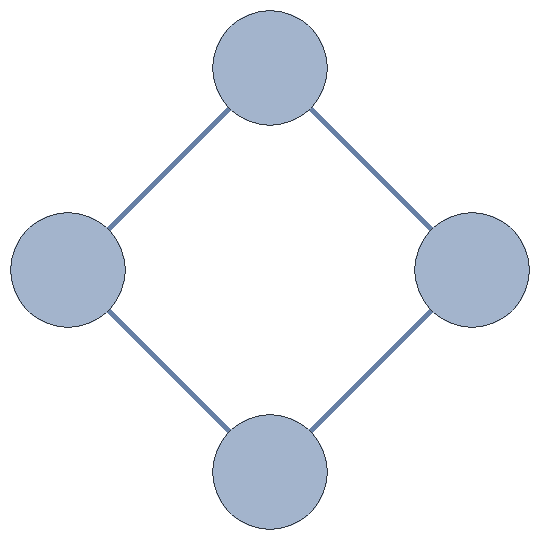
\includegraphics[width=\textwidth]{Images/ring4_nolabels}
		\end{column}
		\begin{column}{0.33\textwidth}
			\centering
    		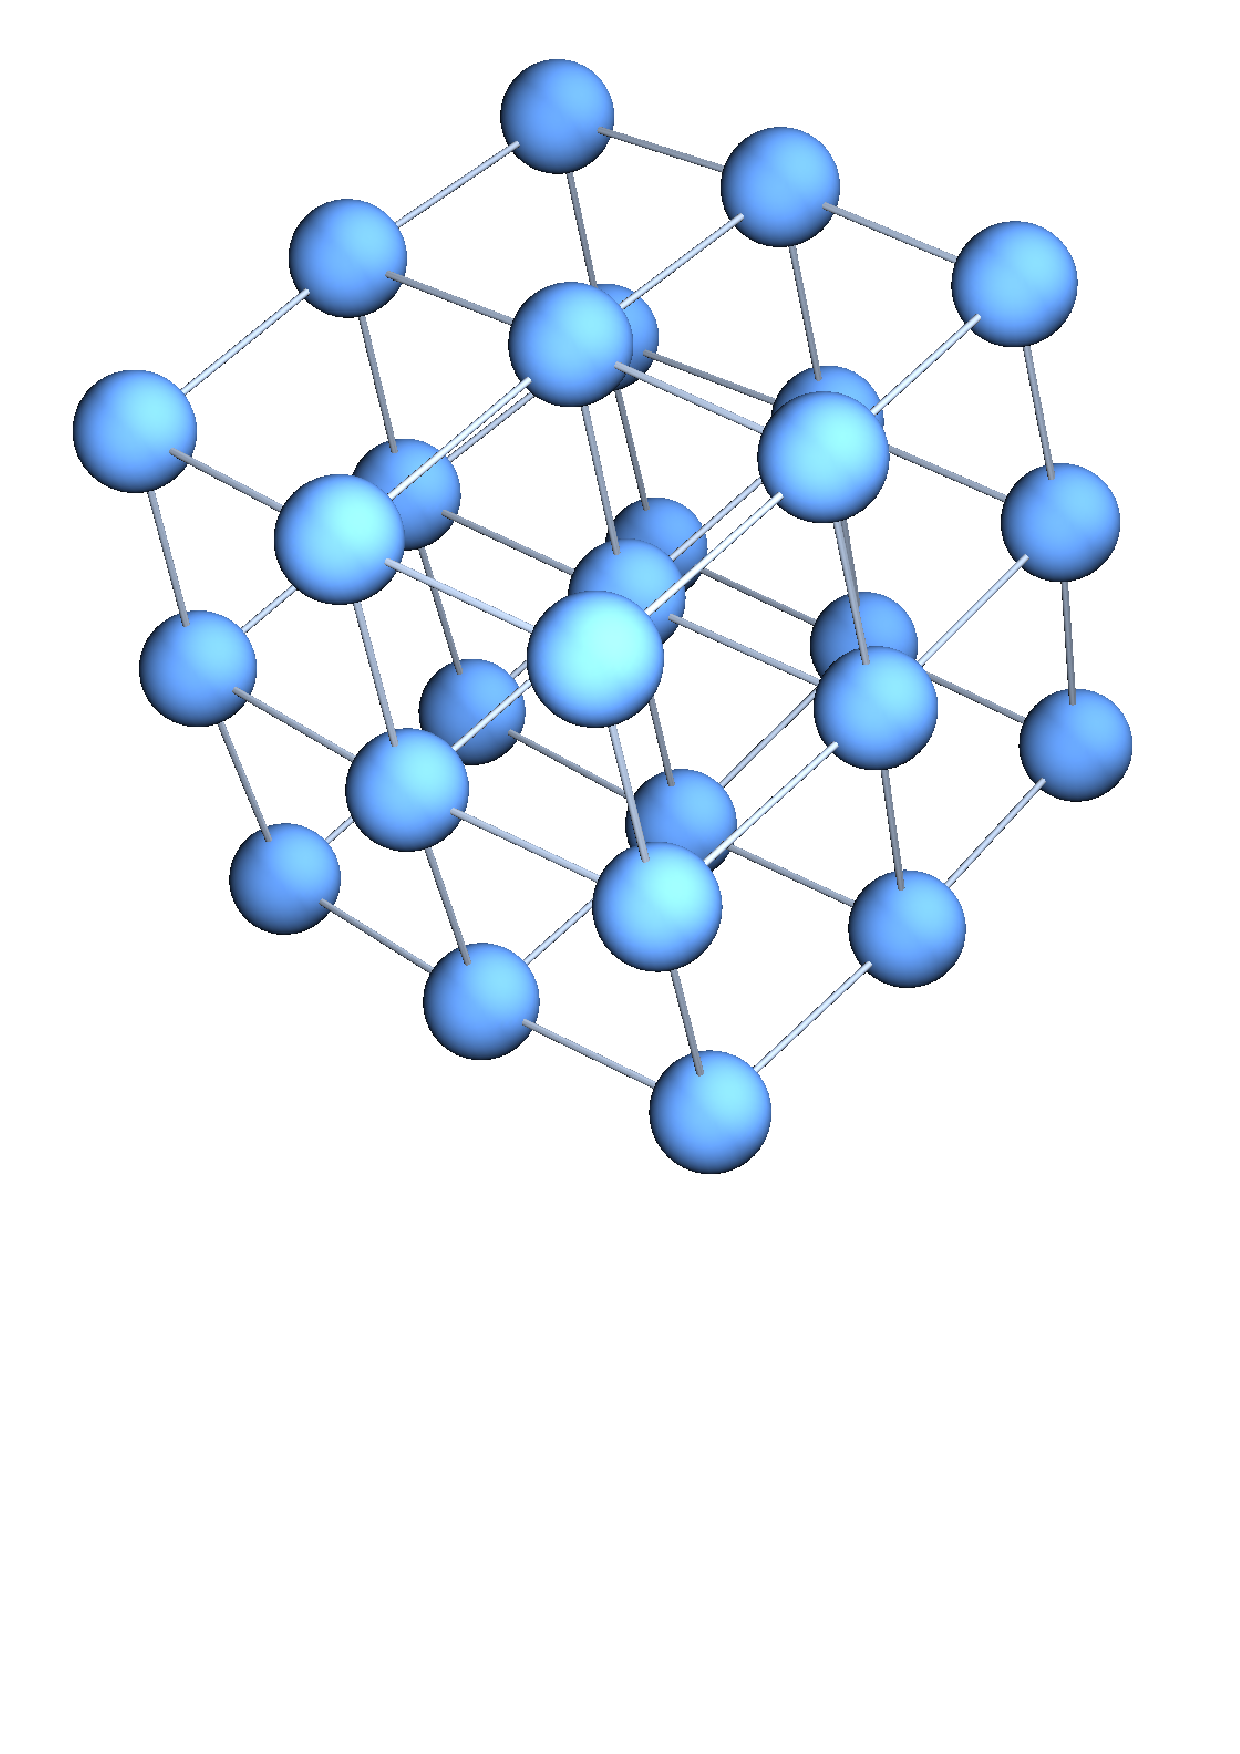
\includegraphics[trim=0 0 0 -10mm, width=\textwidth]{Images/chain3_cubic}\\
    		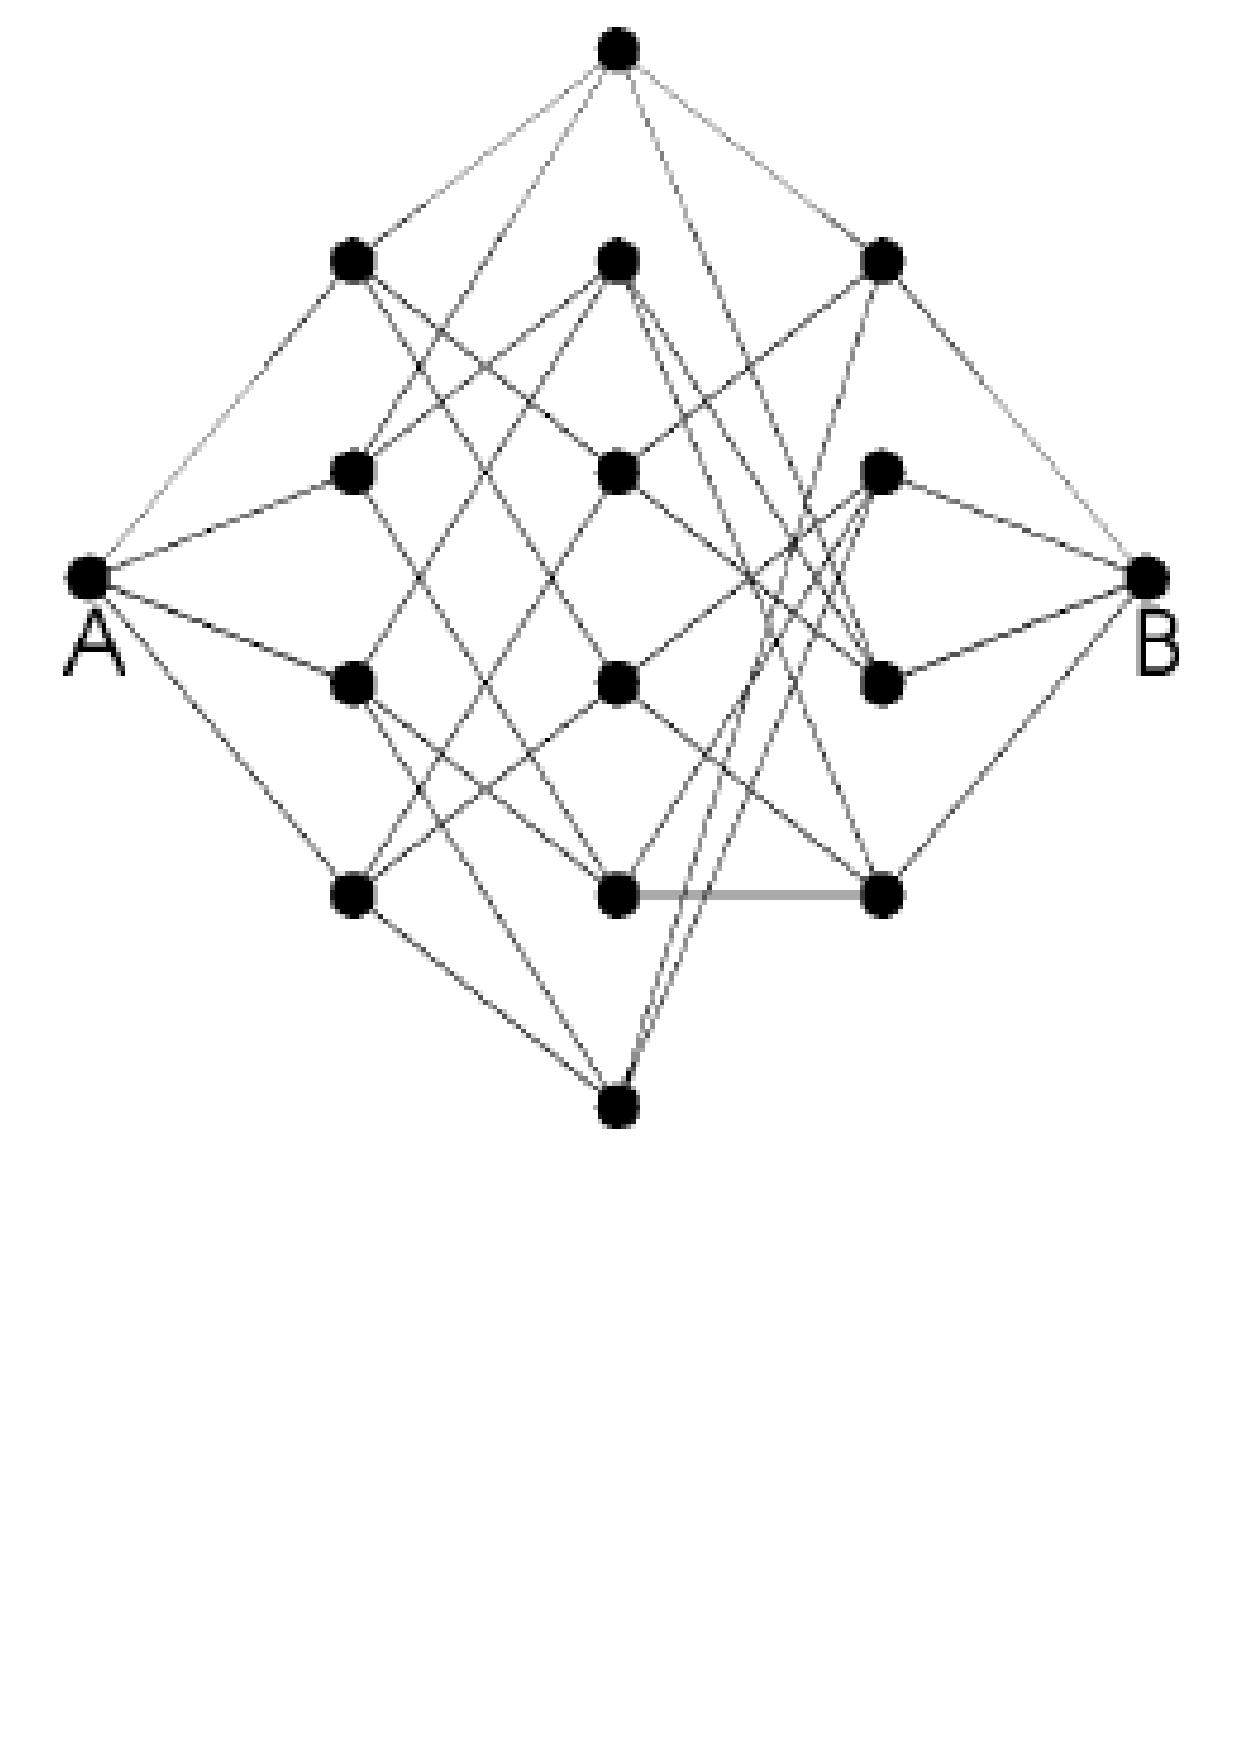
\includegraphics[trim=0 0 0 70mm, width=\textwidth]{Images/chain3_cubic_flattened}
		\end{column}
     	\begin{column}{0.33\textwidth}
     		\centering
     		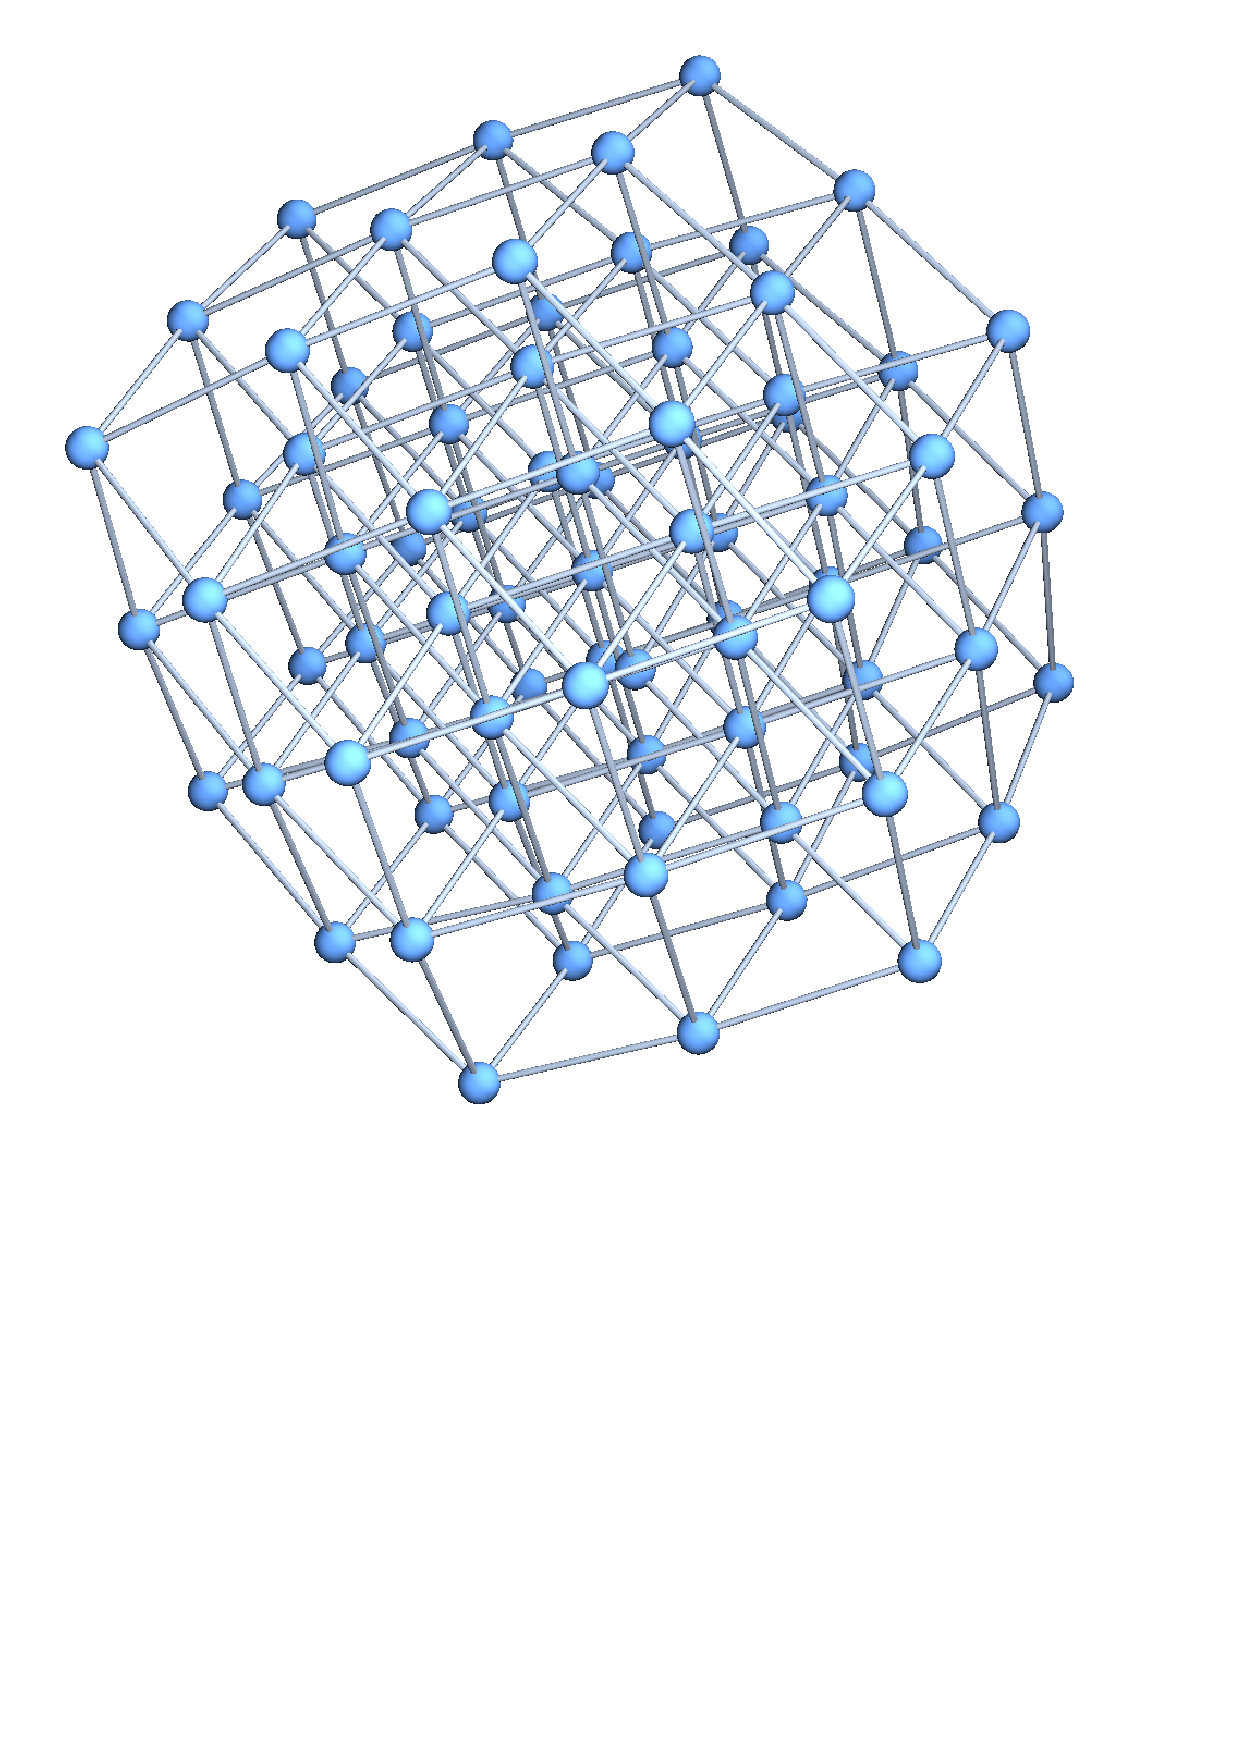
\includegraphics[trim=30mm 0 0 0, width=\textwidth]{Images/chain3_hypercube}
		\end{column}
	\end{columns}
%    Spin chains too short -> more complex networks, explain kronecker product of graphs, sketch proof for fidelity decomposition, hypercubes, flattened versions.
\end{frame}

Spin structures can be examined by building the expression for the transition amplitude and seeing whether this can equal 1 for some parameters. It turns out that for a simple spin chain, the transition amplitude can only ever be 1 if the chains consists of either 2 or 3 qubits. Higher lenghts are excluded by showing that the ratios of eigenvalue differences of the adjacency matrix/hamiltonian must form rational numbers. This can be analyzed with algebraic numbers.\\
These chains are very short. As explained in the last chapter, the graph product helps covering larger distances. By exploiting symmetry, different sites can be connected at the same time. Connectable sites are antipodal on the graph.

\subsection{Spin Switch}
\begin{frame}[t]{Spin Switch}
	\begin{exampleblock}{}
	\setlength\abovedisplayskip{-8pt}
	\begin{center}
		\[ H = \frac{1}{2}J\sum_{i=2}^{N}\left[\sigma_1^x\sigma_i^x + \sigma_1^y\sigma_i^y\right] + \sum_{i=1}^{N}h_i\sigma_i^z \]
	\end{center}
	\end{exampleblock}
	\begin{columns}[T]
		\begin{column}{0.5\textwidth}
			\centering
   			\begin{itemize}
				\item Introduce local potentials
				\item Slight variations only
				\item Diagonal entries 
				\item E.g. magnetic offset field
			\end{itemize}
		\end{column}
		\begin{column}{0.5\textwidth}
			\centering
    		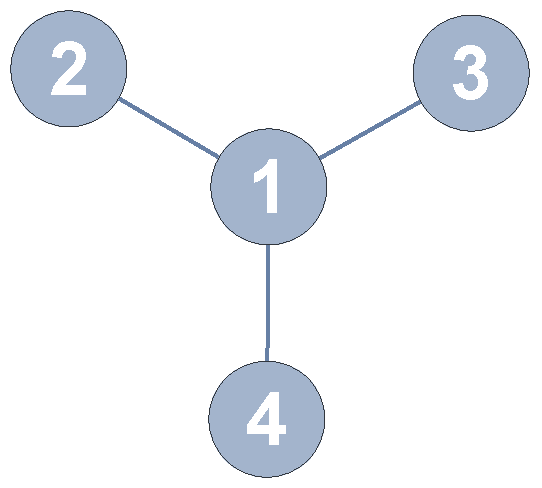
\includegraphics[trim=0mm 0 0 0mm, width=0.8\textwidth]{Images/switch_labeled}
		\end{column}
	\end{columns}
%    Pic of Switch, Variety low, introduce local potentials, only affect diagonal entries, add loops to vertices (left out for clarity), realized as magnetic fields etc.
\end{frame}

\begin{frame}{Spin Switch}
	\begin{columns}[T]
		\begin{column}{0.6\textwidth}
   			\centering
   			\begin{itemize}
   				\item Start: $\ket{\Psi_1} = \alpha \ket{0} + \beta \ket{2}$
   				\item Target: $\ket{\Psi_2} = \alpha \ket{0} + \beta \ket{3}$
   				\item $\braket{3|U(\tau)|2} = \braket{2|U(\tau)|3} \mbeq 1$
   				\item Set $h_2 = h_3$, since $\left[H,P_{23}\right]=0$ 
   				%\[U(\tau)=\sum_{k=0}^3\ket{e_k}\bra{e_k}e^{-\text{i}E_k\tau}\]
   			\end{itemize}
		\end{column}
		\begin{column}{0.4\textwidth}
			\centering
    		$H = \begin{pmatrix}
			h_1 & 1 & 1 & 1 \\
			1 & h_2 & 0 & 0 \\
			1 & 0 & h_3 & 0 \\
			1 & 0 & 0 & h_4
\end{pmatrix}$
		\end{column}
	\end{columns}
	\[\sum_{k=1}^4\bra{2}(P_{23}\ket{e_k})\braket{e_k|2}e^{-\text{i}E_k\tau} \mbeq 1\]\\
   			Choose $E_k$ so they eliminate the phase introduced by $P_{23}$: $E_k \in \{0,h_2,\pm\eta h_2\}$, $\eta$ even.\\
   			Compare $\det(H-\lambda\text{1}_4) = 0$ and $\det(\text{diag}(0,h_2,\pm\eta h_2)-\lambda\text{1}_4) = 0$\\
   			Real roots of the resulting polynomial are solutions for $h_2$, $\tau = \frac{\pi}{h_2}$.
%    sketch calculation, more arms handled by renormalization, fidelities
\end{frame}

\begin{frame}{Spin Switch with more Arms}
			\begin{itemize}
			\item Impose further symmetry condition: $\lambda_4 = \lambda_5 = \dots = \lambda_N$
			\item Renormalize $\ket{4}_{new}=(\ket{4}_{old} + \ket{5} + \dots + \ket{N})/\sqrt{M}$, $M=N-3$
			\end{itemize}
	\begin{columns}
		\begin{column}{0.5\textwidth}
   			\centering
   			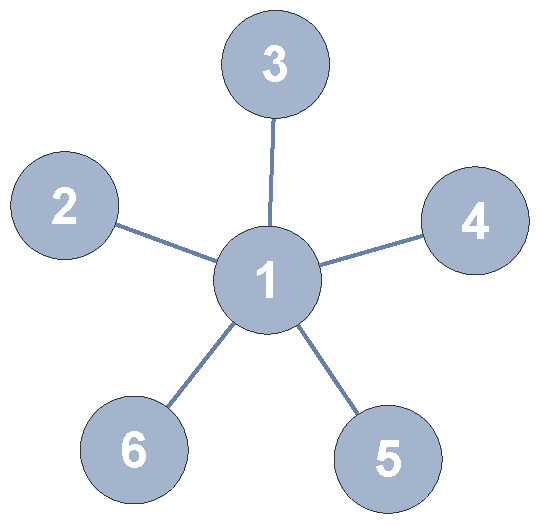
\includegraphics[trim=0mm 0 0 0mm, width=1.2\textwidth]{Images/switch5_labeled}
		\end{column}
		\begin{column}{0.5\textwidth}
			\centering
    		$\tilde{H} = \begin{pmatrix}
			h_1 & 1 & 1 & \sqrt{M} \\
			1 & h_2 & 0 & 0 \\
			1 & 0 & h_3 & 0 \\
			\sqrt{M} & 0 & 0 & h_4
\end{pmatrix}$
		\end{column}
	\end{columns}
%    sketch calculation, more arms handled by renormalization, fidelities
\end{frame}

\begin{frame}[t]{Fidelity}
	\centering
	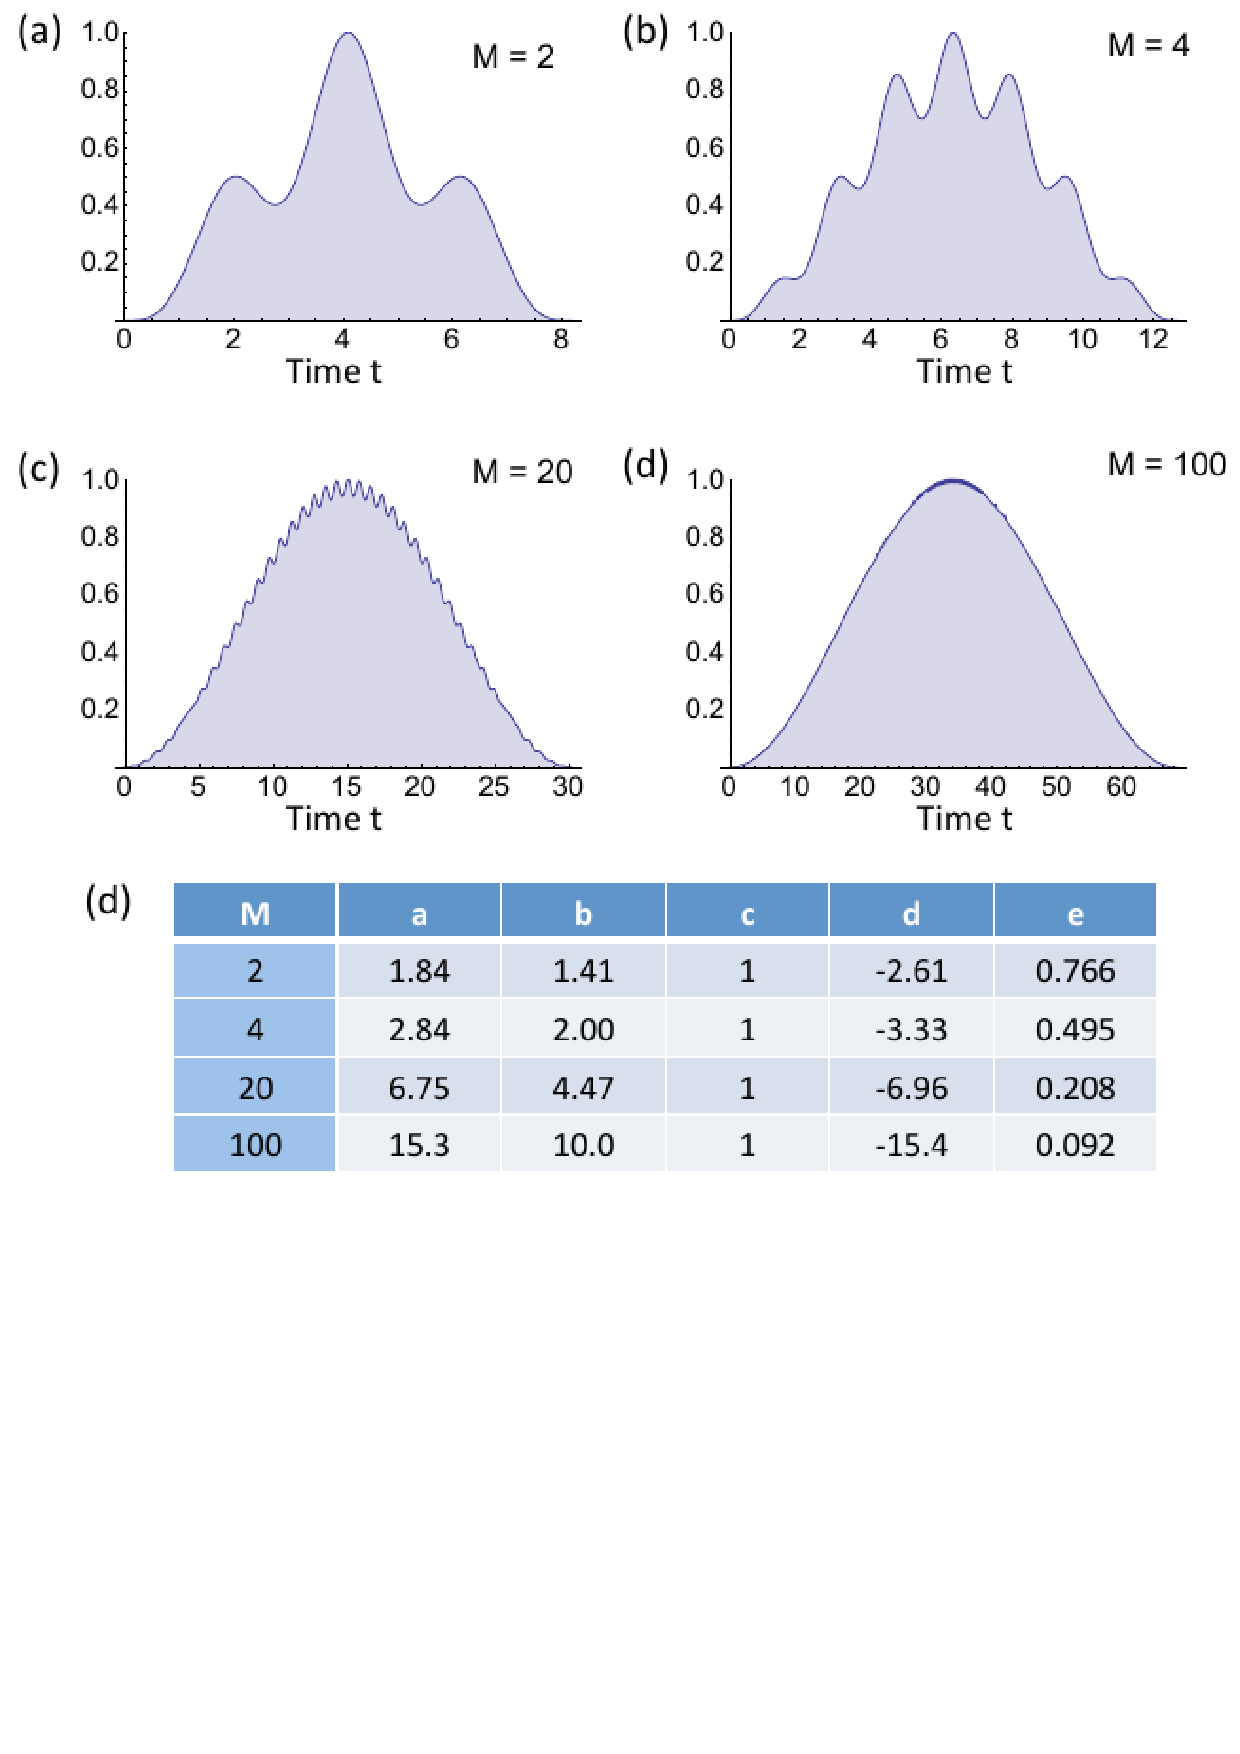
\includegraphics[trim=-20mm 0mm 30mm 0mm, width=0.7\textwidth]{Images/switch_fidelities}
\end{frame}

\subsection{Switch$^2$}
\begin{frame}{Switch$^2$}
	\begin{columns}[T]
		\begin{column}{0.5\textwidth}
			\centering
   			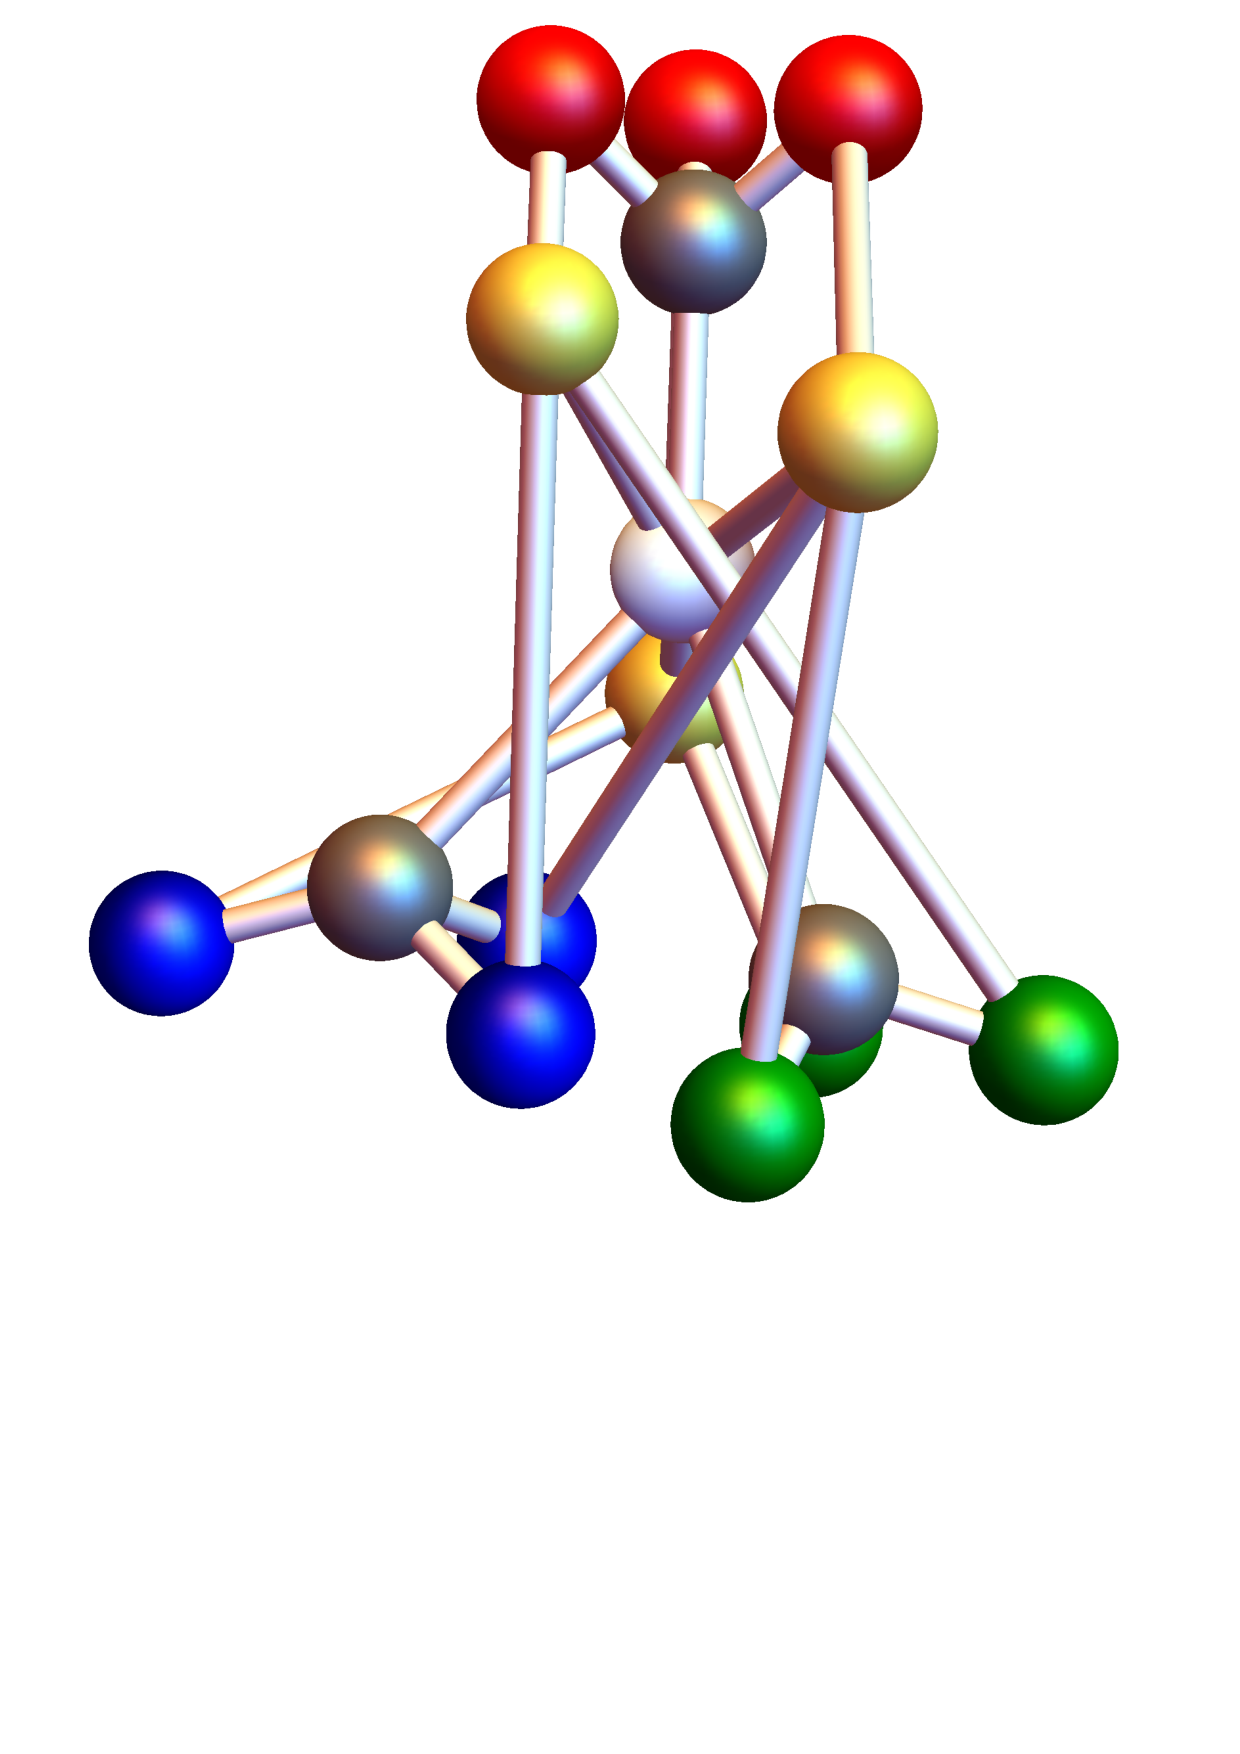
\includegraphics[trim=0mm 0 0 0mm, width=1.2\textwidth]{Images/switch_square}
		\end{column}
		\begin{column}{0.5\textwidth}
			\centering
    		\begin{itemize}
    			\item $h_{u,v} = h_u + h_v \rightarrow $ local potentials are added
    			\item State at vertex $(2,2)$ is transferred to vertex $(3,3)$ or $(4,4)$ at $t = \frac{\pi}{h_2}$
    			\item Symmetry of simple switch $\rightarrow$ transfer from $(2,3)$ to $(3,2)$ or $(2,4)$ to $(4,2)$ with same configuration
    			\item Higher products similar
    		\end{itemize}
		\end{column}
	\end{columns}
%    graph product works with local potentials as well, added at each site, symmetries, more arms.
\end{frame}

It is possible to achieve greater variety in what is possible by introducing local potentials into the model. These might be local magnetic fields, varied slightly by offset fields. In adjacency matrices, these potentials are represented by diagonal elements and form self-loops in graphs. These are omitted for clarity.\\
A first example of what can be achieved with local potentials are spin switches. These are star networks, enabling the input site to decide what arm of the star to transport a state to. The switching is done by applying an offset field, changing the local potentials at each site by a small value. The calculation of these values is an inverse eigenvalue problem. The eigenvalue spectrum is chosen such as to compensate for the eigenvalues of the permutation operator introduced into the transition amplitude.\\
The graph product of this switching network with itself yields a higher order switchable network. The participating nodes are identified by building pairs of the nodes involved in the simple switch graph. The input node is ${2,2}$, able to switch to either ${3,3}$ or ${4,4}$. Using the simple graph's symmetry, the same magnetic configuration enables switching from ${2,3}$ to ${3,2}$ or ${2,4}$ to ${4,2}$ respectively. This graph connects several nodes at the same time. Higher graphs or product graphs of switches with more arms function similarly.

\section{Roadmap}
\subsection{Varying Couplings}
\begin{frame}[t]{Varying Couplings}
	\begin{exampleblock}{}
	\setlength\abovedisplayskip{-8pt}
	\begin{center}
		\[H_{XX}=\frac{1}{2}\sum_{i=1}^{N}{J_i\left[\sigma_i^x\sigma_{i+1}^x + \sigma_i^y\sigma_{i+1}^y\right]}\]
	\end{center}
	\end{exampleblock}
	\begin{columns}[T]
		\begin{column}{0.5\textwidth}
			\centering
			Weighted graphs
   			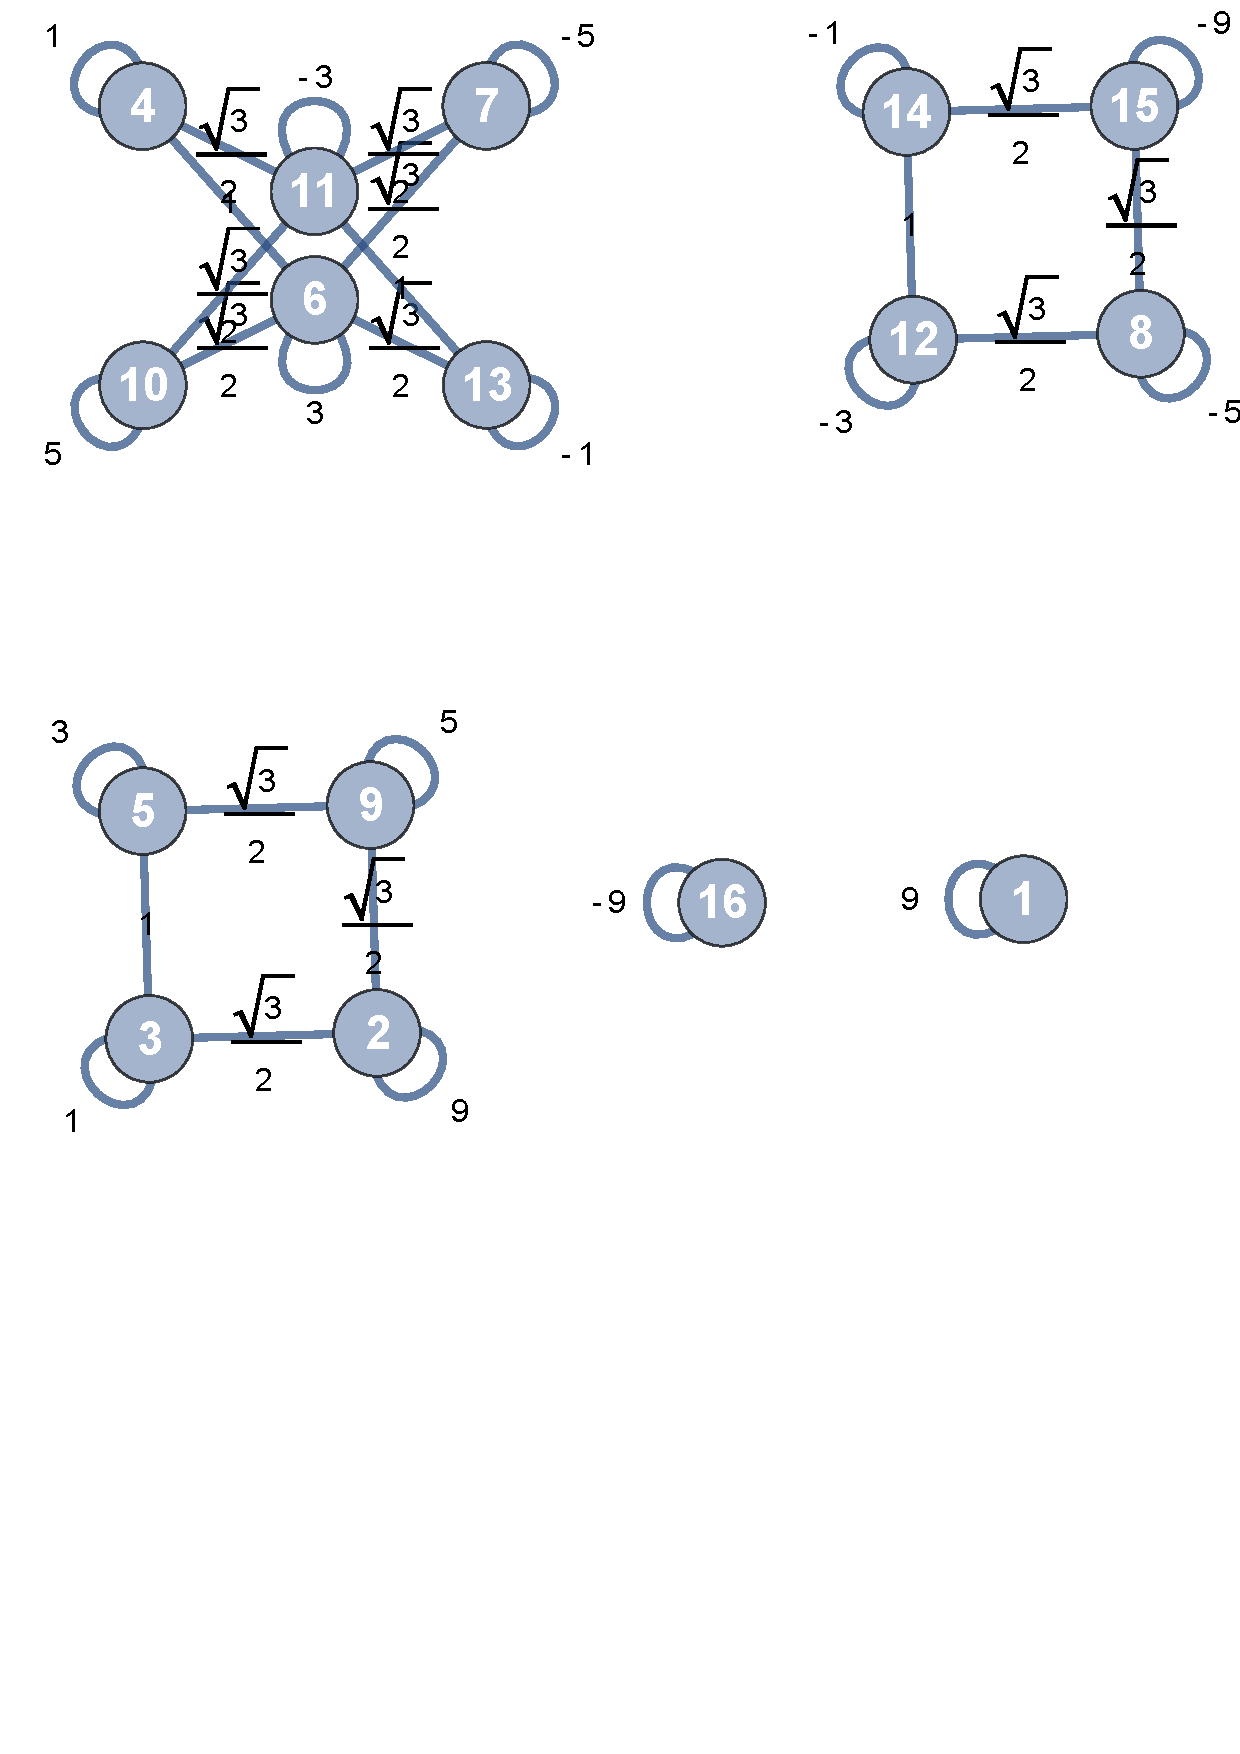
\includegraphics[trim=0mm 0 0 0mm, width=0.8\textwidth]{Images/graph_vary}
		\end{column}
		\begin{column}{0.5\textwidth}
			\centering
			Weighted adjacency matrices
   			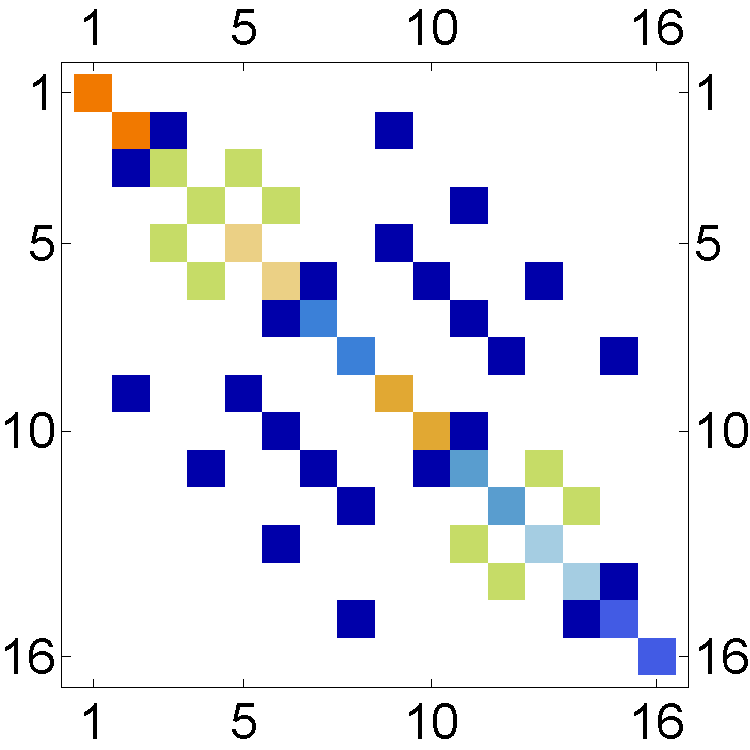
\includegraphics[trim=0mm 0 0 0mm, width=0.7\textwidth]{Images/adj_vary}
		\end{column}
	\end{columns}
	
%    Local couplings leads to much more variety, spin chains with perfect couplings (isomorphism of hilbert spaces to spin n-something particle), not yet looked at switch
\end{frame}

\begin{frame}[t]{Perfect Couplings}
	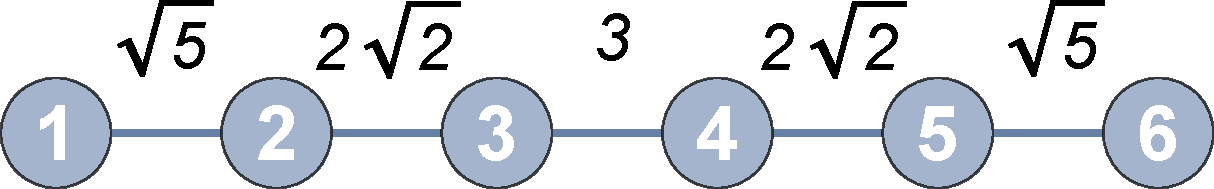
\includegraphics[trim=0mm 0 0 0mm, width=\textwidth]{Images/chain6_perf}
	\begin{itemize}
%		\item Hilbert spaces of same dimensions are isomorphic
		\item Let $J_i = \frac{\lambda}{2}\sqrt{i(N-i)}$
		\item N qubit spin chain with $J_i \leftrightarrow$ Particle with spin $s = \frac{N-1}{2}$ % S_x is angular momentum operator
		\item $H=\lambda S_x \rightarrow U(t)=e^{-\text{i}\lambda t S_x}$
		\item $\braket{N|U(t)|1} = \left( -\text{i}\sin\left(\frac{\lambda t}{2}\right) \right)^{N-1}$
	\end{itemize}	
   	\[H = \begin{pmatrix}
	0 & \sqrt{5} & 0 & 0 & 0 & 0 \\
	\sqrt{5} & 0 & \sqrt{8} & 0 & 0 & 0 \\
	0 & \sqrt{8} & 0 & \sqrt{9} & 0 & 0 \\
	0 & 0 & \sqrt{9} & 0 & \sqrt{8} & 0 \\
	0 & 0 & 0 & \sqrt{8} & 0 & \sqrt{5} \\
	0 & 0 & 0 & 0 & \sqrt{5} & 0 
	\end{pmatrix}\]
%    Local couplings leads to much more variety, spin chains with perfect couplings (isomorphism of hilbert spaces to spin n-something particle), not yet looked at switch also from flattened hypercube
\end{frame}

Even more variety can be achieved by allowing local couplings. These can, in principal, be arbitrary. The hamiltonians of $N$-qubit spin chains and particles of spin $\frac{N-1}{2}$ ($H = \lambda S_x$) share the same structure. The transition amplitude for both turns out to be the same expression, if the couplings for the chain are changed to $J_i = \sqrt{i(N-i)}$. The time evolution operator for this particle is simply a rotation around the x-axis. The matrix elements for this rotation are well-known and can be looked up. The overall transition amplitude equals that of the two qubit chain with an exponent. Therefore, perfect state transfer on a chain coupled according to the above expression is always possible, motivating that these are called perfect couplings.

\subsection{Higher Excitation Subspaces}
\begin{frame}{Higher Excitation Subspaces} %[fragile,t] for listings
	\begin{columns}
		\begin{column}{0.5\textwidth}
			\centering
				\begin{itemize}
		\item PST in larger networks%might be possible for single qubit controlled sites
		\item Control more than one qubit
		\begin{itemize}
			\item Quantum error correction and fault tolerance
		\end{itemize}
		\item Prepare multiple states, send to different target sites
	\end{itemize}
		\end{column}
		\begin{column}{0.5\textwidth}
			\centering
			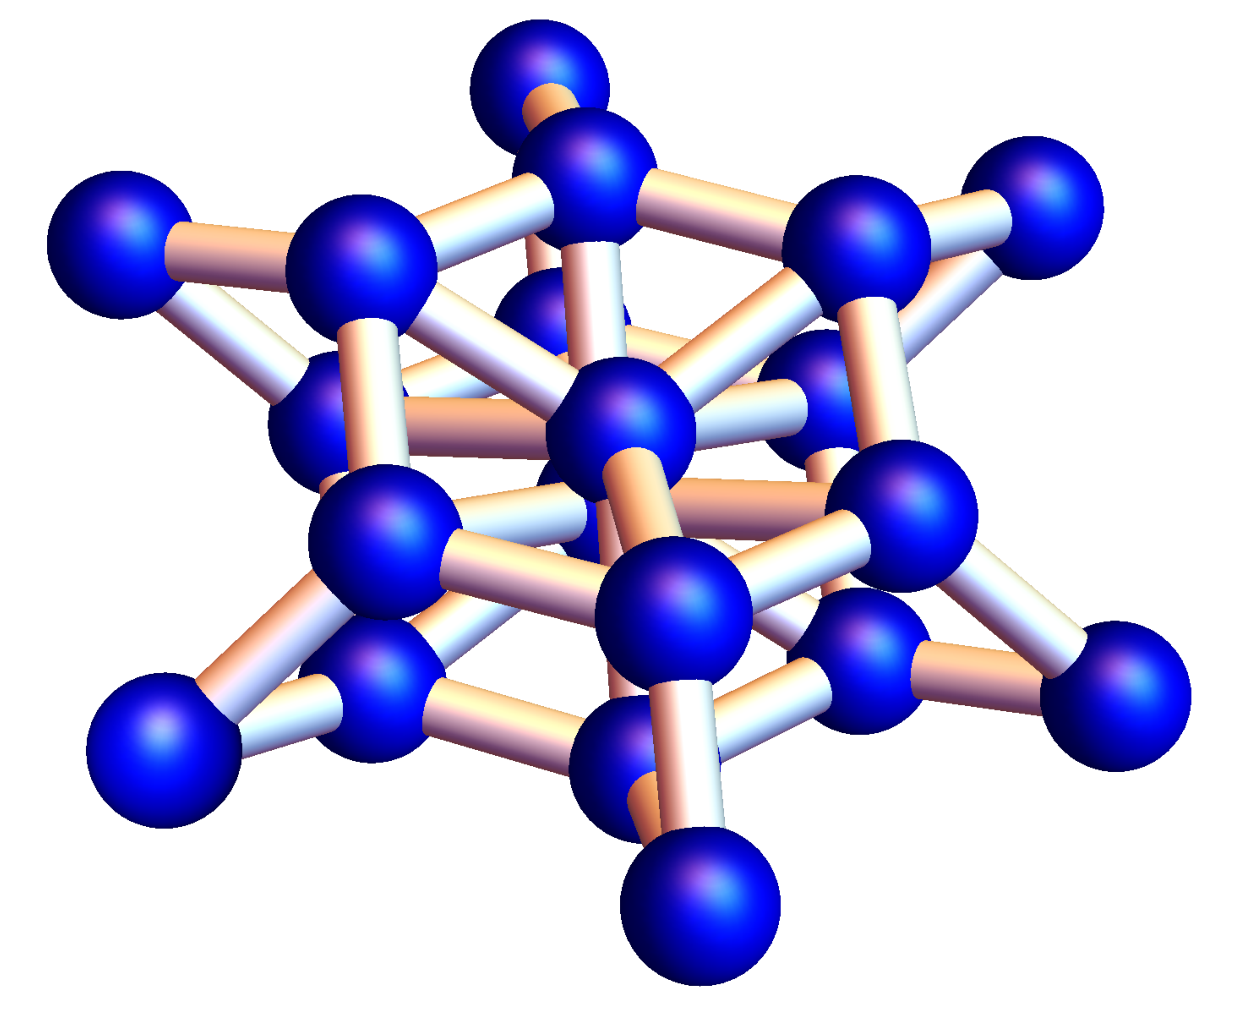
\includegraphics[trim=0mm 0 0 0mm, width=\textwidth]{Images/multispinex}\\
			Calculating higher spin graphs from single spin graphs is an easy task.
		\end{column}
	\end{columns}
	
%	\begin{lstlisting}[language=Python]
%def getEdges(self,spin=1):
%    edges = []
%    for vertex in self.getVertices(spin):
%        dec = self.__decompose(vertex)
%        for comb in combinations(dec,spin-1):
%            neighbours = self.__neighbours([x for x in dec if x not in comb][0])
%            for nn in neighbours:
%                if nn not in comb:
%                    edges += [(vertex,self.__xor(list(comb)+[nn]))]
%        neighbours = []
%    decomposition = []
%    return edges
%	\end{lstlisting}
%    Possibility to control more than one qubit at each site, rings, QEC and fault tolerance, easy to calculate higher spin subspace graphs and hamiltonians, even full hamiltonian
\end{frame}

It might be possible to control multiple qubits at each site, such that quantum error correction is possible. Also, it might turn out (see next slide), that PST is possible in the 2-spin subspace without necessitating control over more than one qubit. If QEC is possible, near perfect state transfer suffices to enable computing. Some implementation of a stabilizer code would flatten the fidelity curves, so that imperfect timing in reading the received qubit state poses no hard risk to successful state transfer.\\
If multiple qubits can be controlled at the same time, networks could be capable of simultaneous state transfer to different sites.\\
Computing higher spin subspace graphs is easily possible by examining next neighbours of single excited spin states and assembling the edges according to these connections. This way, the whole hamiltonian can be rebuilt by starting at the single spin subspace graph, then calculating higher spin graphs up to spin $N$ in an $N$-qubit spin network. The adjacency matrix of all these graphs taken as a single disconnected graph is the complete hamiltonian of the system.

\subsection{Entanglement}
\begin{frame}{Entanglement}
	\begin{center}
		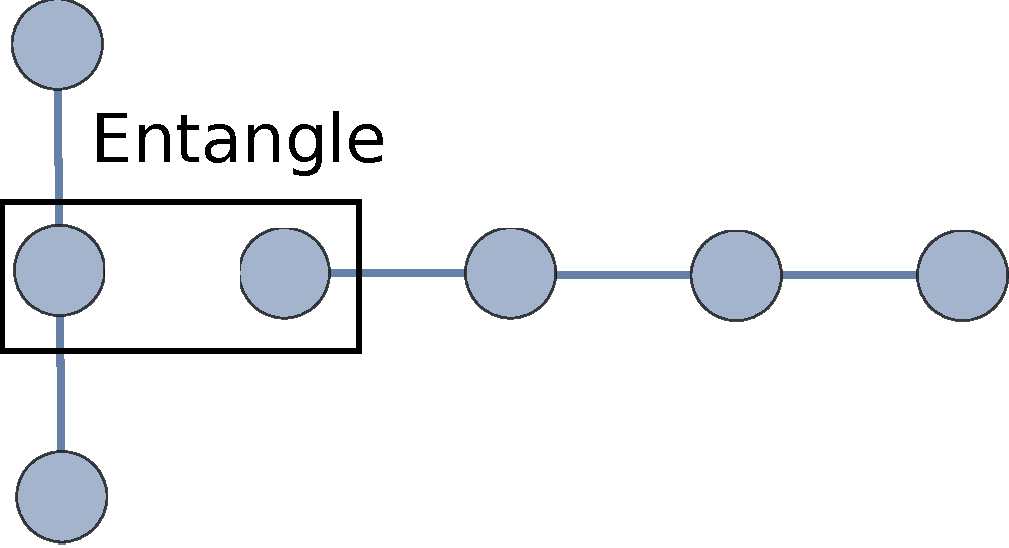
\includegraphics[trim=0mm 0 0 0mm, width=0.5\textwidth]{Images/entanglement}
	\end{center}
	\begin{itemize}
		\item Transport part of an entangled pair along the network
		\item Entangle separated parts of a system
		\item Quantum teleportation as transportation scheme
	\end{itemize}
%    Dynamics of entanglement, teleportation for transport.
\end{frame}

\subsection{Experimental Verification}
\begin{frame}{Experimental Verification}
	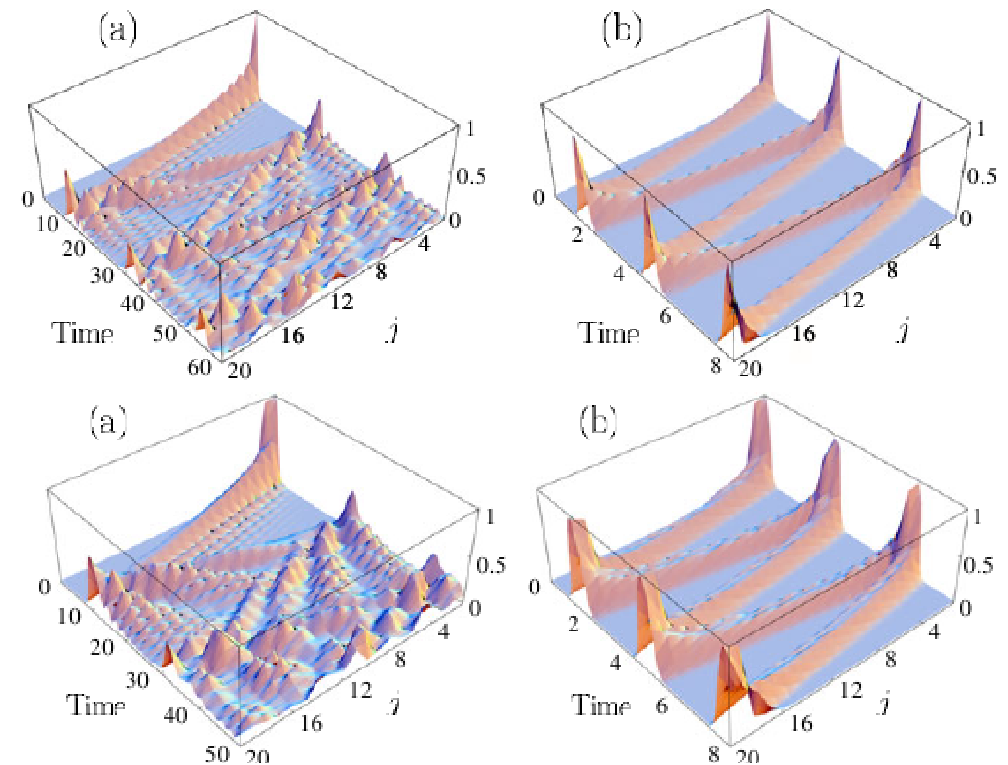
\includegraphics[trim=0mm 0 0 0mm, width=0.9\textwidth]{Images/experiment_chains}
%    Some experiments verify these results, Georgios paper (cm4) for two-spin up subspace analysis and great pictures, quantum dots
\end{frame}

\section{Goal}
\begin{frame}{Goal}
	\begin{itemize}
		\item Framework for engineering spin chains with given properties
		\item Define certain constraints for hamiltonian
		\item Single spin subgraph should yield a network capable of PST
	\end{itemize}
%    Define general constraints on hamiltonians so that the single spin subspace graph leads to a network automatically capable of perfect state transfer, hints: symmetry, EV difference quotient rational, connectivity.
\end{frame}

\end{document}
